\chapter{Superconductors}\label{chap:15}
The gap of a superconductor is more than three thousand times smaller than the gap of silicon. In aluminum $\Delta_{\mathrm{BCS}} = \SI{0.18}{meV}$, so breaking a pair costs \SI{0.36}{meV}, and a dark-matter particle of \SI{0.10}{keV} can break a pair (\cref{we:7-al}). Below a third of an MeV no halo particle can cross the gap of silicon (\cref{sec:1.3}), yet a superconductor still responds to a coupling to the electron density, and the BCS theory gives that response in closed form. The question of this chapter is whether the rate of breaking pairs can be computed as reliably as the semiconductor rates of \cref{chap:10}.

The response of independent quasiparticles, however, violates charge conservation, and the correction that restores it is largest at the small momentum transfers that light dark matter favors (\cref{sec:7.2}). At the edge $\omega = 2\Delta_{\mathrm{BCS}}$ the coherence factors make the absorptive part of the response jump, and the screening that follows from that jump cannot be expanded. And the sensors are thin films, often amorphous and strongly disordered, whereas the BCS model describes a clean bulk crystal. As a result the loss function of aluminum near the edge changes by a factor of 4.6 with the mean free path of the film. Far above the edge, by contrast, the simpler truncations of the response agree with the conserving response to a few percent (\cref{fig:15-map}).

\begin{figure}[tbp]
  \centering
  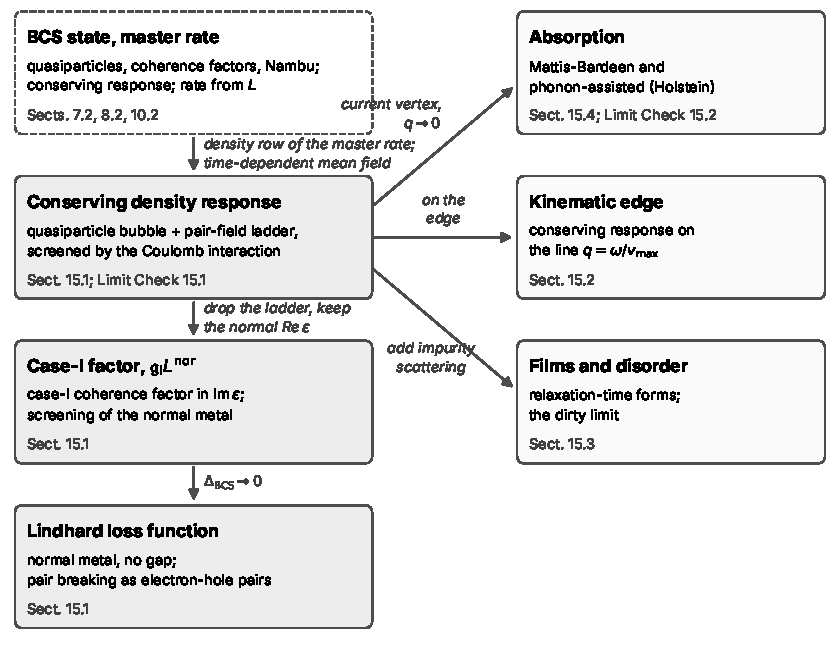
\includegraphics[width=0.85\linewidth]{figures/ch15/map15.pdf}
  \caption{Superconductors, from the BCS state of \cref{sec:7.2} and the loss-function rate of \cref{sec:8.2,sec:10.2} to the targets of this chapter. The density response that conserves charge adds the pair-field ladder to the quasiparticle bubble and is screened by the Coulomb interaction (\cref{sec:15.1}; \cref{lim:15.1a}). Dropping the ladder and keeping the screening of the normal metal leaves the case-I coherence factor times the normal loss function; letting the gap close leaves the Lindhard function of the normal metal (\cref{sec:15.1}). On the kinematic edge $q = \omega/v_{\mathrm{max}}$ each truncation is worst (\cref{sec:15.2}). Impurity scattering and the film geometry change the response of real sensors (\cref{sec:15.3}). At vanishing momentum the current and the spin current give the absorption of dark photons and axion-like particles, with and without a phonon (\cref{sec:15.4}; \cref{lim:15.4a}).}
  \label{fig:15-map}
\end{figure}

\section{Pair breaking by dark matter}\label{sec:15.1}

A dark-matter particle of \SI{1}{keV} that scatters in aluminum deposits at most \SI{3.5}{meV}, about ten times the pair-breaking threshold, and transfers at most \SI{5.3}{eV} of momentum. To deposit $\omega$ it must transfer at least $q = \omega/v_{\mathrm{max}}$, with $v_{\mathrm{max}} = 2.650\times10^{-3}$ the largest speed of a halo particle in the laboratory (\cref{eq:1.2-vmax}). The line $q = \omega/v_{\mathrm{max}}$ in the $(q,\omega)$ plane, the \emph{kinematic edge}, is a different object from the \emph{pair-breaking edge} $\omega = 2\Delta_{\mathrm{BCS}}$, the threshold in energy. The ratio of the gap to the Doppler width of the Fermi surface is $\Delta_{\mathrm{BCS}}/qv_{\mathrm{F}} = (v_{\mathrm{max}}/v_{\mathrm{F}})(\Delta_{\mathrm{BCS}}/\omega)$, and it takes its largest value on the kinematic edge, 0.20 at the threshold. \Cref{sec:7.2} found that this ratio controls the correction that restores charge conservation. We build the loss function from the conserving response of \cref{eq:7.2-Rc}. Two truncations of the conserving response are accurate far above the pair-breaking edge: the Lindhard function of the normal metal, and the same function multiplied by the case-I coherence factor of \cref{eq:7.2-pairspec}.

\subsection{The loss-function rate of a superconductor}\label{sec:15.1-rate}

A mediator that couples to the electron number acts through the density row of the master formula, with $\mathfrak{D}_{ee} = |\tilde V(\vect{q})|^2$ and $S = (2q^2/e^2)\,L/(1 - \ee^{-\beta\omega})$ (\cref{sec:10.2}). At \SI{10}{mK} the threshold has $\beta\omega = 418$, so the thermal factor is one, and the spectrum is \cref{eq:10.2-rate} with $\bar L$ replaced by the loss function of the superconductor, which is isotropic in the model used here. For a dark photon, which couples to the total charge, this spectrum is exact. For a mediator that couples to electrons alone it holds with the nuclei clamped, and the lattice then enters only through the pairing interaction already contained in $\Delta_{\mathrm{BCS}}$. The ions' own response appears in the loss function through the phonon pole at $\omega = c_{\mathrm{LA}}q$, and above that pole the ionic response is a correction of relative order $(c_{\mathrm{LA}}q/\omega)^2$. The longitudinal sound speed along [100] is $c_{\mathrm{LA}} = (C_{11}/\rho)^{1/2} = \SI{6.47}{km.s^{-1}}$, from the zero-temperature elastic constant $C_{11} = \SI{114.3}{GPa}$~\cite[Table~2]{malica2020quasi} and the low-temperature density $\rho = \SI{2.73}{g.cm^{-3}}$. The correction is then $(c_{\mathrm{LA}}/v_{\mathrm{max}})^2 = \num{6.6e-5}$ on the kinematic edge. For $\mchi < \SI{3.2}{keV}$ even the largest momentum transfer, $2\mchi v_{\mathrm{max}}$, excites phonons only below $2\Delta_{\mathrm{BCS}}$.

The dielectric function is the proper density response screened by the Coulomb interaction, $\varepsilon = 1 - v_{\mathrm{C}}(q)\tilde R$ (\cref{sec:4.4}). In the normal metal the random-phase approximation puts the independent-particle bubble in place of $\tilde R$, and the result is the Lindhard function of \cref{eq:4.5-rpa}. In the superconductor, however, the proper response must itself conserve charge, and \cref{sec:7.2} showed that the bare quasiparticle bubble does not. The conserving response is the time-dependent mean field in the three Nambu channels $(\boldsymbol{\eta}, \mathsf{s}_1, \mathsf{s}_2)$ of \cref{eq:7.2-nambu}, the pair-field ladder of \cref{eq:7.2-Rc}~\cite{anderson1958random}. In field-theory language the ladder is the vertex correction that restores the Ward identity of charge. Adding the Coulomb interaction in the density channel gives the generalized random-phase approximation:
\begin{keyresult}[Conserving loss function of a superconductor]
\begin{equation}
  \varepsilon^{\mathrm{cons}}(q,\omega) = 1 - v_{\mathrm{C}}(q)\,R^{\mathrm{cons}}(q,\omega), \qquad
  L^{\mathrm{cons}}(q,\omega) = \Imag\Bigl[-\frac{1}{\varepsilon^{\mathrm{cons}}(q,\omega)}\Bigr] ,
  \label{eq:15.1-Lcons}
\end{equation}
with $R^{\mathrm{cons}} = R_{\boldsymbol{\eta}\boldsymbol{\eta}}$ the density response of \cref{eq:7.2-Rc}, which contains the pair-field ladder and no Coulomb interaction.
\end{keyresult}
\noindent The Coulomb interaction is a function of the local density and commutes with it, so the screened response obeys the continuity equation and the f-sum rule whenever $R^{\mathrm{cons}}$ does (\cref{sec:7.2}). The core electrons of aluminum add a constant of order one to $\varepsilon$, negligible against $k_{\mathrm{TF}}^2/q^2 \ge \num{5.8e5}$ for $q \le \SI{5.3}{eV}$. Here $k_{\mathrm{TF}} = \SI{4.05}{keV}$ is the Thomas--Fermi wavevector of the free-electron gas of aluminum: three electrons per atom in the fcc cell of side $a = \SI{4.05}{\angstrom}$, so $\nd_e = \SI{1.81e23}{cm^{-3}}$, $k_{\mathrm{F}} = \SI{1.75}{\angstrom^{-1}}$, the bare electron mass, $v_{\mathrm{F}} = k_{\mathrm{F}}/m_e = \num{6.75e-3}$ and $\omega_p = \SI{15.78}{eV}$. The amplitude channel $\mathsf{s}_1$ decouples from the density in a metal whose density of states is symmetric about the Fermi level (\cref{sec:7.2}); the asymmetry over the energy range of the pairs is of relative order $\Delta_{\mathrm{BCS}}/E_{\mathrm{F}} = \num{1.5e-5}$, and we drop it.

\subsection{The conserving response in closed form}\label{sec:15.1-closed}

For aluminum we set the temperature to zero, take the density of states $\mathcal{N}_{\mathrm{F}}$ constant over the energies of the pairs, and take the metal clean. We also linearize the band across the shell, $\xi_{\vect{k}+\vect{q}} = \xi_{\vect{k}} + v_{\mathrm{F}}q\mu$ with $\mu$ the cosine of the angle between $\vect{k}$ and $\vect{q}$. The dropped term $q^2/2m_e$ is below \SI{3e-5}{eV} for $q \le \SI{5.3}{eV}$, whereas $v_{\mathrm{F}}q \ge 2.5\,\omega$. With these simplifications every bubble of \cref{eq:7.2-Rc} reduces to one function. At $T = 0$ the density and pair operators either create a pair of quasiparticles, with energy $E + E'$ for $E = E_{\vect{k}}$ and $E' = E_{\vect{k}+\vect{q}}$, or destroy one, and the bubbles are
\begin{equation}
  R^0_{AB}(q,\omega) = \frac{1}{\Vol}\sum_{\vect{k}}\Bigl[\frac{M^{\mathrm{N}*}_AM^{\mathrm{N}}_B}{\omega - E - E' + \ii0^+} - \frac{M^{\mathrm{N}}_AM^{\mathrm{N}*}_B}{\omega + E + E' + \ii0^+}\Bigr] ,
  \label{eq:15.1-bubble}
\end{equation}
with $M^{\mathrm{N}}_A$ the amplitude with which the Nambu-channel operator $O_A$ (superscript N for Nambu) creates the pair. For the density it is $M^{\mathrm{N}}_{\boldsymbol{\eta}} = uv' + vu'$ of \cref{eq:7.2-coh}. The phase operator is $O_{\mathsf{s}_2} = -\ii(B^\dagger_{\vect{q}} - B_{-\vect{q}})$, with $B^\dagger_{\vect{q}}$ the pair creation operator of \cref{app:D.21}. It therefore creates the same pair through $B^\dagger_{\vect{q}}$, with the amplitude $M^{\mathrm{N}}_{\mathsf{s}_2} = -\ii(uu' + vv')$; this phase reproduces $R^0_{\mathsf{s}_2\boldsymbol{\eta}}$ of \cref{sec:7.2} at $q = 0$, and the sign of the ladder below does not depend on it. With \cref{eq:7.2-E},
\begin{gather*}
  |M^{\mathrm{N}}_{\boldsymbol{\eta}}|^2 = \frac{EE' - \xi\xi' + \Delta_{\mathrm{BCS}}^2}{2EE'}, \qquad
  |M^{\mathrm{N}}_{\mathsf{s}_2}|^2 = \frac{EE' + \xi\xi' + \Delta_{\mathrm{BCS}}^2}{2EE'}, \\
  M^{\mathrm{N}*}_{\boldsymbol{\eta}}M^{\mathrm{N}}_{\mathsf{s}_2} = -\frac{\ii\Delta_{\mathrm{BCS}}(E + E')}{2EE'} ,
\end{gather*}
where the mixed product follows from $(uv' + vu')(uu' + vv') = u'v'(u^2 + v^2) + uv(u'^2 + v'^2) = \Delta_{\mathrm{BCS}}/2E' + \Delta_{\mathrm{BCS}}/2E$.

The linear band turns these three products into functions of $E + E'$. Since $E^2 = \xi^2 + \Delta_{\mathrm{BCS}}^2$, the product $(EE' + \xi\xi' + \Delta_{\mathrm{BCS}}^2)(EE' - \xi\xi' - \Delta_{\mathrm{BCS}}^2) = E^2E'^2 - (\xi\xi' + \Delta_{\mathrm{BCS}}^2)^2$ equals $\Delta_{\mathrm{BCS}}^2(\xi' - \xi)^2$, and $EE' + \xi\xi' + \Delta_{\mathrm{BCS}}^2$ is half of $(E + E')^2 - (\xi' - \xi)^2$. For the density amplitude we write $EE' - \xi\xi' + \Delta_{\mathrm{BCS}}^2 = (EE' - \xi\xi' - \Delta_{\mathrm{BCS}}^2) + 2\Delta_{\mathrm{BCS}}^2$ and use the product for the first bracket. With $\xi' - \xi = v_{\mathrm{F}}q\mu$,
\begin{equation}
  EE' + \xi\xi' + \Delta_{\mathrm{BCS}}^2 = \tfrac12\bigl[(E + E')^2 - v_{\mathrm{F}}^2q^2\mu^2\bigr], \qquad
  |M^{\mathrm{N}}_{\boldsymbol{\eta}}|^2 = \frac{\Delta_{\mathrm{BCS}}^2(E + E')^2}{EE'\bigl[(E + E')^2 - v_{\mathrm{F}}^2q^2\mu^2\bigr]} .
  \label{eq:15.1-ident}
\end{equation}
The quantity $\omega_\mu^2 = \omega^2 - v_{\mathrm{F}}^2q^2\mu^2$ is the energy of the pair in the frame that moves with the Doppler shift, and a pair at angle $\mu$ can be created only if $\omega_\mu \ge 2\Delta_{\mathrm{BCS}}$, the counterpart of the threshold \cref{eq:7.2-threshold}. The remaining integral is the $q = 0$ pair sum $F(\omega)$ of \cref{sec:7.2}, now at each angle. A hyperbolic substitution evaluates it (\cref{app:D.39}):
\begin{equation}
  F_\mu(\omega) = \frac{\mathcal{N}_{\mathrm{F}}}{2}\int\dd\xi\,\frac{E + E'}{EE'\,\bigl[\omega^2 - (E + E')^2\bigr]}
  = -\frac{\mathcal{N}_{\mathrm{F}}}{2\Delta_{\mathrm{BCS}}^2}\,\frac{\arcsin\sqrt{\mathfrak{p}_\mu}}{\sqrt{\mathfrak{p}_\mu(1 - \mathfrak{p}_\mu)}}, \qquad
  \mathfrak{p}_\mu = \frac{\omega_\mu^2}{4\Delta_{\mathrm{BCS}}^2} ,
  \label{eq:15.1-F}
\end{equation}
for $0 < \mathfrak{p}_\mu < 1$, with $F_0 = F$, and continued to the other ranges of $\mathfrak{p}_\mu$ in \cref{eq:D.39-Fcont}. Only at $\mathfrak{p}_\mu > 1$, where pairs can be created, is $F_\mu$ complex.

The density bubble follows from \cref{eq:15.1-bubble,eq:15.1-ident} with $\Vol^{-1}\sum_{\vect{k}} \to \mathcal{N}_{\mathrm{F}}\int\dd\xi\int_{-1}^1\dd\mu/2$. Splitting the integrand of the density bubble by partial fractions into an $F_\mu$ term and an elementary term, and using the gap equation, gives (\cref{app:D.39}), with $\langle X\rangle_\mu = \int_0^1\dd\mu\,X$,
\begin{equation}
  \begin{gathered}
  R^0_{\boldsymbol{\eta}\boldsymbol{\eta}} = \Bigl\langle\frac{2\mathcal{N}_{\mathrm{F}}v_{\mathrm{F}}^2q^2\mu^2 + 4\Delta_{\mathrm{BCS}}^2\omega^2F_\mu}{\omega_\mu^2}\Bigr\rangle_\mu, \\
  R^0_{\mathsf{s}_2\boldsymbol{\eta}} = -R^0_{\boldsymbol{\eta}\mathsf{s}_2} = 2\ii\Delta_{\mathrm{BCS}}\,\omega\,\langle F_\mu\rangle_\mu, \qquad
  1 + \tfrac12V_{\mathrm{BCS}}R^0_{\mathsf{s}_2\mathsf{s}_2} = \tfrac12V_{\mathrm{BCS}}\langle\omega_\mu^2F_\mu\rangle_\mu .
  \end{gathered}
  \label{eq:15.1-bubbles}
\end{equation}
At $q = 0$ these three expressions are the bubbles of \cref{sec:7.2}. The last expression is the denominator of the phase channel in \cref{eq:7.2-Rc}, and the coupling $V_{\mathrm{BCS}}$ drops out of the result:
\begin{keyresult}[Conserving density response of a clean superconductor]
\begin{equation}
  R^{\mathrm{cons}}(q,\omega) = \underbrace{\Bigl\langle\frac{2\mathcal{N}_{\mathrm{F}}v_{\mathrm{F}}^2q^2\mu^2 + 4\Delta_{\mathrm{BCS}}^2\omega^2F_\mu(\omega)}{\omega^2 - v_{\mathrm{F}}^2q^2\mu^2}\Bigr\rangle_\mu}_{\text{bare bubble } R^0_{\boldsymbol{\eta}\boldsymbol{\eta}}}
  \;\underbrace{-\;\frac{4\Delta_{\mathrm{BCS}}^2\omega^2\,\langle F_\mu(\omega)\rangle_\mu^2}{\langle(\omega^2 - v_{\mathrm{F}}^2q^2\mu^2)F_\mu(\omega)\rangle_\mu}}_{\text{pair-field ladder}} ,
  \label{eq:15.1-Rcons}
\end{equation}
with $F_\mu$ of \cref{eq:15.1-F}, for $T = 0$, constant $\mathcal{N}_{\mathrm{F}}$, a linear band and no impurities.
\end{keyresult}
\noindent At $q = 0$ the ladder cancels the bubble for every $\omega$, as \cref{eq:7.2-cancel} states. At small $q$ the cancellation is incomplete, and $R^{\mathrm{cons}} \to 2\mathcal{N}_{\mathrm{F}}v_{\mathrm{F}}^2q^2/3\omega^2 = \nd_eq^2/m_e\omega^2$, the free-particle tail whose coefficient is the f-sum rule; at $v_{\mathrm{F}}q = 0.01\,\Delta_{\mathrm{BCS}}$, $R^{\mathrm{cons}}$ and the free-particle tail agree to one part in $10^5$, while the bare bubble stays at its $q = 0$ value. At $\omega \to 0$ the bubble gives $-2\mathcal{N}_{\mathrm{F}}$, the Thomas--Fermi value, and the ladder vanishes: pairing leaves the static screening of the metal unchanged. As $\Delta_{\mathrm{BCS}} \to 0$ at fixed $\omega/qv_{\mathrm{F}}$, the conserving response approaches the Lindhard function at $q \ll k_{\mathrm{F}}$, to \num{6e-5} at $v_{\mathrm{F}}q = 10^3\,\Delta_{\mathrm{BCS}}$ and \num{8e-7} at $10^4\,\Delta_{\mathrm{BCS}}$.

Below $2\Delta_{\mathrm{BCS}}$ no pairs can be created, $F_\mu$ is real, and $L^{\mathrm{cons}}$ vanishes except where $\varepsilon^{\mathrm{cons}}$ does. The denominator of the ladder vanishes at one frequency $\varOmega_{\mathrm{AB}}(q) < 2\Delta_{\mathrm{BCS}}$: the Anderson--Bogoliubov mode of \cref{sec:7.2}, the Goldstone mode of the broken phase symmetry, now at finite $q$. There $R^{\mathrm{cons}}$ has a pole, so $\varepsilon^{\mathrm{cons}}$ has one too and the loss function has a zero, not a peak. The Coulomb interaction moves the weight of the mode to the plasmon, as \cref{sec:7.2} anticipated (the Anderson--Higgs mechanism), and a sum rule proves that no loss weight is left below $2\Delta_{\mathrm{BCS}}$ (\cref{app:D.39}). Through the Kramers--Kronig relation the pole still shifts $\Real\varepsilon^{\mathrm{cons}}$ above $2\Delta_{\mathrm{BCS}}$. On the kinematic edge at $\omega = 2.2\,\Delta_{\mathrm{BCS}}$, the pole term alone exceeds the whole shift of $\Real\varepsilon^{\mathrm{cons}}$ relative to the Lindhard function, and there the rest of the ladder acts the other way. The pole term is \SI{58}{\percent} of the shift at $2.5\,\Delta_{\mathrm{BCS}}$, \SI{16}{\percent} at $3\Delta_{\mathrm{BCS}}$, and zero at $5\Delta_{\mathrm{BCS}}$, where the edge momentum has pushed the mode into the pair continuum. The pole explains the shift only for $y \lesssim 2.3$.

The clean limit needs only $\mathcal{N}_{\mathrm{F}}$, $v_{\mathrm{F}}$ and $\Delta_{\mathrm{BCS}}$, and no first-principles calculation.

\subsection{The case-I coherence factor}\label{sec:15.1-bare}

Without the ladder the density response is the bare bubble $R^0_{\boldsymbol{\eta}\boldsymbol{\eta}}$, with the dielectric function $\varepsilon^{\mathrm{bare}} = 1 - v_{\mathrm{C}}R^0_{\boldsymbol{\eta}\boldsymbol{\eta}}$. The absorptive part of $\varepsilon^{\mathrm{bare}}$ comes from the imaginary part of $F_\mu$ alone, $\Imag F_\mu = -\pi\mathcal{N}_{\mathrm{F}}/[4\Delta_{\mathrm{BCS}}^2\sqrt{\mathfrak{p}_\mu(\mathfrak{p}_\mu - 1)}]$ for $\omega_\mu > 2\Delta_{\mathrm{BCS}}$. Changing the variable of the angular average from $\mu$ to $\omega_\mu$, $\dd\mu = -\omega_\mu\,\dd\omega_\mu/[v_{\mathrm{F}}q(\omega^2 - \omega_\mu^2)^{1/2}]$, gives
\begin{equation*}
  \Imag R^0_{\boldsymbol{\eta}\boldsymbol{\eta}} = -\frac{4\pi\mathcal{N}_{\mathrm{F}}\Delta_{\mathrm{BCS}}^2\omega^2}{v_{\mathrm{F}}q}\int_{2\Delta_{\mathrm{BCS}}}^{\omega}\frac{\dd\omega'}{\omega'^2\sqrt{\omega'^2 - 4\Delta_{\mathrm{BCS}}^2}\,\sqrt{\omega^2 - \omega'^2}} ,
\end{equation*}
provided $v_{\mathrm{F}}q \ge (\omega^2 - 4\Delta_{\mathrm{BCS}}^2)^{1/2}$, so that the whole interval of $\omega_\mu$ lies inside $0 \le \mu \le 1$. The normal metal has $\Imag R^0 = -\pi\mathcal{N}_{\mathrm{F}}\omega/v_{\mathrm{F}}q$ below $\omega = qv_{\mathrm{F}}$ (\cref{sec:4.5}). The ratio of the superconducting to the normal absorptive part depends on $y = \omega/\Delta_{\mathrm{BCS}}$ alone:
\begin{keyresult}[Absorptive part of the bare quasiparticle bubble]
\begin{equation}
  \begin{gathered}
  \Imag\varepsilon^{\mathrm{bare}}(q,\omega) = \mathfrak{g}_{\mathrm{I}}\Bigl(\frac{\omega}{\Delta_{\mathrm{BCS}}}\Bigr)\,\Imag\varepsilon_{\mathrm{Lin}}(q,\omega) \qquad \bigl(v_{\mathrm{F}}q \ge (\omega^2 - 4\Delta_{\mathrm{BCS}}^2)^{1/2}\bigr), \\
  \mathfrak{g}_{\mathrm{I}}(y) = 4y\int_2^y\frac{\dd u}{u^2\sqrt{u^2 - 4}\sqrt{y^2 - u^2}} = \Bigl(1 + \frac{2}{y}\Bigr)\mathrm{E}(k) - \frac{4\,\mathrm{K}(k)}{y + 2}, \qquad k = \frac{y - 2}{y + 2} ,
  \end{gathered}
  \label{eq:15.1-gI}
\end{equation}
with $\mathrm{K}$ and $\mathrm{E}$ the complete elliptic integrals of the first and second kind of modulus $k$, for $y > 2$; $\mathfrak{g}_{\mathrm{I}} = 0$ below.
\end{keyresult}
\noindent The function $\mathfrak{g}_{\mathrm{I}}$ is the case-I ratio $S_{\mathrm{I}}/S_{\mathrm{n}}$ of \cref{eq:7.2-pairspec}, obtained there by counting pairs in the energies of the two quasiparticles and here by integrating over the angle; the two integrals agree with the elliptic form to $10^{-12}$. It jumps to $\pi/2$ at $y = 2$, is 1.322 at $y = 3$ and 1.051 at $y = 10$, and \cref{tab:15-edge} lists it at the other energies we use. Allen's theory of phonon-assisted absorption in metals contains the elliptic form~\cite{allen1971electron}, as quoted by Hochberg, Lin and Zurek~\cite[Eq.~(17)]{hochberg2016absorption}. The corresponding case-II form is that of Mattis and Bardeen~\cite{mattis1958theory}. Under the simplifications above, \cref{eq:15.1-gI} is exact: the absorptive part of the bare bubble carries no correction in powers of $\Delta_{\mathrm{BCS}}/qv_{\mathrm{F}}$. The validity condition of \cref{eq:15.1-gI} holds for every momentum transfer of halo dark matter, since $v_{\mathrm{F}}q \ge v_{\mathrm{F}}\omega/v_{\mathrm{max}} = 2.5\,\omega$.

The pair-field ladder changes the absorptive part. Its relative size is the vertex fraction $\mathfrak{v} = \Imag(R^{\mathrm{cons}} - R^0_{\boldsymbol{\eta}\boldsymbol{\eta}})/\Imag R^0_{\boldsymbol{\eta}\boldsymbol{\eta}}$, which follows from \cref{eq:15.1-Rcons} by quadrature over $\mu$ (\cref{app:D.39}). On the kinematic edge the vertex fraction is largest near the threshold, $+0.44$ at $y = 2.2$, and falls to $+0.004$ at $y = 10$ (\cref{tab:15-edge}). The vertex fraction does not fall monotonically with $q$, however: at $y = 5$ it is $+0.052$ on the edge and still $+0.044$ at four times the edge momentum, and at $y = 10$ it is nearly three times larger at that momentum than on the edge.

At the threshold itself the ladder replaces the jump of \cref{eq:7.2-pairspec} by a steep rise. The bare absorptive part jumps to $\pi/2$ times the normal value at $y = 2$; in the conserving response it starts from zero and rises steeply. At the edge momentum of $y = 2.05$, $\Imag\varepsilon^{\mathrm{cons}}/\Imag\varepsilon_{\mathrm{Lin}}$ is 0.14 at $y - 2 = 10^{-6}$, 0.64 at $10^{-3}$ and 1.30 at $10^{-2}$, and it passes the bare value $\pi/2$ before $y - 2 = 0.03$, that is within \SI{5}{\micro eV} of the threshold. For a rate integrated over energy, the conserving response therefore keeps a step at $2\Delta_{\mathrm{BCS}}$, smoothed over a few microelectronvolts. The conserving loss function vanishes at $2\Delta_{\mathrm{BCS}}$ with its absorptive part and is back to $0.97\,L^{\mathrm{nor}}$ by $y - 2 = 0.03$, with $L^{\mathrm{nor}} = \Imag[-1/\varepsilon_{\mathrm{Lin}}]$.

\begin{figure}[tbp]
  \centering
  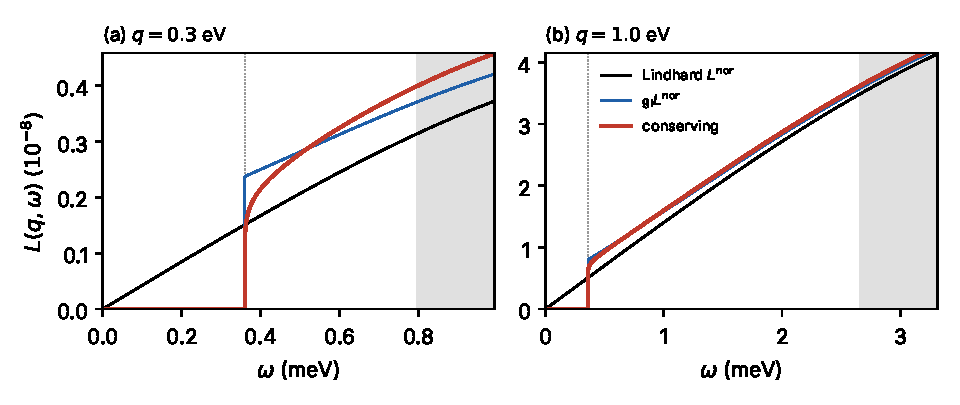
\includegraphics[width=\linewidth]{figures/ch15/fig15_1.pdf}
  \caption{Loss function of aluminum near the pair-breaking edge at the momentum transfers (a) $q = \SI{0.3}{eV}$ and (b) $q = \SI{1}{eV}$, against the energy $\omega$, for the bulk gap $\Delta_{\mathrm{BCS}} = \SI{0.18}{meV}$ (dotted line at $2\Delta_{\mathrm{BCS}}$). Red: conserving response, \cref{eq:15.1-Lcons,eq:15.1-Rcons}; blue: the case-I factor times the normal loss function, $\mathfrak{g}_{\mathrm{I}}L^{\mathrm{nor}}$; black: Lindhard loss function of the normal metal, $L^{\mathrm{nor}}$. Halo dark matter reaches the energies left of the gray band, $\omega \le qv_{\mathrm{max}}$. All curves are clean, $T = 0$, with a constant density of states, $v_{\mathrm{F}} = \num{6.75e-3}$ and $k_{\mathrm{TF}} = \SI{4.05}{keV}$. At \SI{0.3}{eV} and $\omega \ge 2.2\,\Delta_{\mathrm{BCS}}$ the conserving loss function lies 27 to \SI{34}{\percent} above the Lindhard function. At \SI{1}{eV} all three agree within \SI{5}{\percent} at the largest reachable energy.}
  \label{fig:15-alloss}
\end{figure}

At $q = \SI{0.3}{eV}$, $v_{\mathrm{F}}q = 11\,\Delta_{\mathrm{BCS}}$, every energy that halo dark matter can deposit lies within $4.4\,\Delta_{\mathrm{BCS}}$ of zero, and the conserving response lies above the Lindhard function (\cref{fig:15-alloss}). At $q = \SI{1}{eV}$, $v_{\mathrm{F}}q = 38\,\Delta_{\mathrm{BCS}}$, the differences between the three loss functions are confined to the first few $\Delta_{\mathrm{BCS}}$ above the edge.

\subsection{Truncations of the conserving response}\label{sec:15.1-chain}

Keeping the case-I absorptive part \cref{eq:15.1-gI} but screening it with the normal metal gives $\Imag\varepsilon^{\mathrm{bare}}/|\varepsilon_{\mathrm{Lin}}|^2 = \mathfrak{g}_{\mathrm{I}}L^{\mathrm{nor}}$~\cites[Eq.~(10)]{gan2026mean}[Eq.~(2) and text]{hochberg2023directional}. Closing the gap, $\Delta_{\mathrm{BCS}} \to 0$ at fixed $\omega$, leaves the Lindhard loss function~\cite[Eqs.~(1), (S.13)]{hochberg2021determining}, whose unscreened structure factor below $qv_{\mathrm{F}}$ is the free-gas $S_{\mathrm{n}} = m_e^2\omega/\pi q$ of \cref{sec:7.2}~\cite[Eq.~(3.4)]{hochberg2016detecting}. Dropping the ladder and keeping the normal real part are both controlled by $\Delta_{\mathrm{BCS}}/qv_{\mathrm{F}}$. Closing the gap is controlled by $y$ alone, through $\mathfrak{g}_{\mathrm{I}}(y) - 1$. On the kinematic edge both controlling parameters, $\Delta_{\mathrm{BCS}}/qv_{\mathrm{F}}$ and $\mathfrak{g}_{\mathrm{I}}(y) - 1$, are functions of $y$, and each truncation is worst on that edge. Over all momentum transfers that halo dark matter reaches, the clean conserving loss function lies between 0.980 and 1.085 times $\mathfrak{g}_{\mathrm{I}}L^{\mathrm{nor}}$ for $y \ge 3$; \cref{sec:15.2} gives the values on the edge, and \cref{sec:15.3-sc} the change with the mean free path.

\begin{limitbox}[Loss function of a superconductor near the pair-breaking edge][lim:15.1a]
Lindhard loss function $L^{\mathrm{nor}}$ in the rate \cref{eq:10.2-rate}, with $\Imag\varepsilon_{\mathrm{Lin}} = (\pi/2)(k_{\mathrm{TF}}^2/q^2)(\omega/qv_{\mathrm{F}})$ below $qv_{\mathrm{F}}$~\cites[Eqs.~(1), (S.13)]{hochberg2021determining}[Eq.~(3.4)]{hochberg2016detecting}; with the case-I factor, $\mathfrak{g}_{\mathrm{I}}L^{\mathrm{nor}}$~\cites[Eq.~(10)]{gan2026mean}[Eq.~(2) and text]{hochberg2023directional}.
\par\smallskip
{\centering
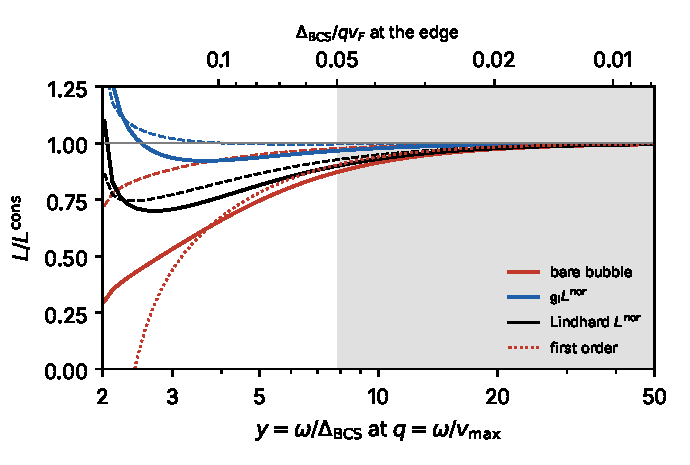
\includegraphics[width=0.92\linewidth]{figures/ch15/limit15_1a.pdf}
\captionof{figure}{Loss function of aluminum on the kinematic edge $q = \omega/v_{\mathrm{max}}$ in two truncations, divided by the conserving loss function \cref{eq:15.1-Lcons}, against $y = \omega/\Delta_{\mathrm{BCS}}$ (top axis: $\Delta_{\mathrm{BCS}}/qv_{\mathrm{F}} = 0.392/y$ there). Blue: $\mathfrak{g}_{\mathrm{I}}L^{\mathrm{nor}}$; black: Lindhard $L^{\mathrm{nor}}$. Dashed: the same at four times the edge momentum. Clean, $T = 0$, constant density of states, $v_{\mathrm{F}} = \num{6.75e-3}$. ``Within \SI{10}{\percent}'' means that the smaller of the two loss functions is at least 0.9 of the larger. Gray: $y \ge 7.9$, where the Lindhard function is within \SI{10}{\percent} of the conserving result on the edge and at all larger momenta. The product $\mathfrak{g}_{\mathrm{I}}L^{\mathrm{nor}}$ is within \SI{10}{\percent} already for $y \ge 2.25$.}\label{fig:15-limit-chain}
\par}
\smallskip
Below $y \approx 3$ on the edge the Lindhard function falls about \SI{30}{\percent} below the conserving loss function, and the clean conserving result itself assumes that impurities do not scatter the electrons within the size of a pair (\cref{sec:15.3-dirty}).
\end{limitbox}

\Cref{fig:15-limit-chain} orders the truncations. The Lindhard function, which has no gap, is within \SI{10}{\percent} of the conserving result for $y \ge 7.9$ on the edge, where $\Delta_{\mathrm{BCS}}/qv_{\mathrm{F}} \le 0.050$, and for $y \ge 6.3$ at four times the edge momentum. At $y = 5$ the Lindhard function is 0.815 of the conserving value on the edge, and the case-I factor $\mathfrak{g}_{\mathrm{I}}(5) = 1.15$ of the conserving response accounts for most of this deficit.

These comparisons are all clean-limit statements. Near the edge the curves are separated by the steep rise of the conserving absorption over a few microelectronvolts, a structure narrower than $\Delta_{\mathrm{BCS}}$. Impurity scattering, at a rate given by $v_{\mathrm{F}}$ over the mean free path, smooths the rise once that rate is no longer small compared with the width of the rise. For $y \ge 3$ the curves depend on functions of $y$ that vary on the scale of $\Delta_{\mathrm{BCS}}$ itself.

\subsection{The aluminum gap and the rate}\label{sec:15.1-al}

The gap enters the loss function through $y = \omega/\Delta_{\mathrm{BCS}}$, in $\mathfrak{g}_{\mathrm{I}}$ and in the ladder, and not only through the threshold. For bulk aluminum it is measured, $\Delta_{\mathrm{BCS}} = \SI{0.18}{meV}$~\cite[Table~III]{savrasov1996electron}, and it agrees within one percent with the weak-coupling value $1.764\,T_c = \SI{0.179}{meV}$ for the measured $T_c = \SI{1.18}{K}$ (\cref{we:7-al}). The value $\Delta = \SI{0.3}{meV}$ often taken for aluminum~\cite[p.~2]{hochberg2023directional} is the film convention $2\Delta_{\mathrm{BCS}} = \SI{0.6}{meV}$ of \cref{sec:1.5}, 1.67 times the bulk value. The film value describes thin films, whose critical temperatures exceed the bulk critical temperature and in ultraclean films approach twice it~\cite{yeh2023doubling}. A rate for a bulk crystal uses \SI{0.18}{meV}. A rate for a film uses the gap measured on that film, and \cref{sec:15.3} adds what the film changes in the response itself.

\begin{workedexample}{The aluminum rate at \SI{1}{keV} with the bulk and the film gap}\label{we:15-alrate}
Take $\mchi = \SI{1}{keV}$, a light mediator, $\FDM = (\alpha m_e/q)^2$, the reference cross section $\sigmae = \SI{e-40}{cm^2}$, the standard halo of \cref{sec:1.2}, and aluminum with $\rho_T = \SI{2.70}{g.cm^{-3}}$, $v_{\mathrm{F}} = \num{6.75e-3}$ and $k_{\mathrm{TF}} = \SI{4.05}{keV}$. The particle deposits at most $\frac12\mchi v_{\mathrm{max}}^2 = \SI{3.51}{meV}$, which is $19.5\,\Delta_{\mathrm{BCS}}$ for the bulk gap and $11.7\,\Delta_{\mathrm{BCS}}$ for the film gap, and transfers at most $2\mchi v_{\mathrm{max}} = \SI{5.30}{eV}$, so that $q/k_{\mathrm{TF}} \le \num{1.3e-3}$ and $v_{\mathrm{F}}q \le 199\,\Delta_{\mathrm{BCS}}$ (bulk). Every point lies in the regime of \cref{eq:15.1-Rcons}.

\Cref{eq:10.2-rate} with the conserving loss function, integrated numerically over $2\Delta_{\mathrm{BCS}} \le \omega \le \SI{3.51}{meV}$ and over the momenta with $\vmin \le v_{\mathrm{max}}$ (Gauss--Legendre sums, in $\omega$ graded toward $2\Delta_{\mathrm{BCS}}$ and in $q$ between the two roots of $\vmin(q,\omega) = v_{\mathrm{max}}$), gives
\begin{equation*}
  \mathcal{R} = \SI{3.26}{kg^{-1}.yr^{-1}}\ (\Delta_{\mathrm{BCS}} = \SI{0.18}{meV}), \qquad
  \mathcal{R} = \SI{2.65}{kg^{-1}.yr^{-1}}\ (\Delta_{\mathrm{BCS}} = \SI{0.30}{meV}) .
\end{equation*}
The bulk gap raises the rate by a factor of 1.23. The lower threshold alone would raise the rate more: with the Lindhard function cut at $2\Delta_{\mathrm{BCS}}$, which has no coherence factor, the factor is 1.30. The difference between the two factors comes from the edge. With the film gap the window $2\Delta_{\mathrm{BCS}} < \omega < 3\Delta_{\mathrm{BCS}}$, where $\mathfrak{g}_{\mathrm{I}}$ is largest, carries \SI{37}{\percent} of the conserving rate; with the bulk gap it carries \SI{20}{\percent}. For a heavy mediator, $\FDM = 1$, the rate at the same cross section is \SI{3.8e-13}{kg^{-1}.yr^{-1}}, and the bulk gap raises it by 1.13.

The choice of loss function matters less than the choice of gap. With the bulk gap and the light mediator, $\mathfrak{g}_{\mathrm{I}}L^{\mathrm{nor}}$ gives 1.010 of the conserving rate, and the Lindhard function cut at the threshold gives 0.850. The normal metal with no gap gives 1.024: at this mass the pile-up of pair states above $2\Delta_{\mathrm{BCS}}$ almost exactly replaces the rate lost below it. With the film gap the same ratios are 1.027, 0.806 and 1.26. These ratios are clean-limit values, and the part of the rate below $3\Delta_{\mathrm{BCS}}$ is the part that impurity scattering can change (\cref{sec:15.3}).
\end{workedexample}

\section{Screening at the kinematic edge}\label{sec:15.2}

A particle at the threshold mass $m_{\mathrm{min}} = \SI{0.10}{keV}$ of \cref{we:7-al} must move at $v_{\mathrm{max}}$ and give up its whole kinetic energy, which takes the momentum transfer $q = m_{\mathrm{min}}v_{\mathrm{max}} = 2\omega/v_{\mathrm{max}}$, twice the edge value. Heavier particles can deposit the same energy with less momentum: from $v_{\mathrm{min}}(q,\omega) = v_{\mathrm{max}}$ the smallest momentum transfer at $\omega = 2\Delta_{\mathrm{BCS}}$ is 1.17 times the edge value for $2m_{\mathrm{min}}$ and only 1.03 times it at \SI{1}{keV}. For every particle a few times heavier than $m_{\mathrm{min}}$, the scatters just above $2\Delta_{\mathrm{BCS}}$ therefore lie close to the kinematic edge.

\subsection{The normal dielectric function on the edge}\label{sec:15.2-resum}

At $q \ll k_{\mathrm{F}}$ the Lindhard function \cref{eq:4.5-lindhard} depends on $\omega$ and $q$ only through the reduced frequency $\mathfrak{w} = \omega/qv_{\mathrm{F}}$, the common limit of the arguments $\omega/qv_{\mathrm{F}} \pm q/2k_{\mathrm{F}}$ as $q/2k_{\mathrm{F}} \to 0$. To first order in $q/k_{\mathrm{F}}$ the bracket of \cref{eq:4.5-lindhard} is the derivative $\partial_{\mathfrak{w}}[(1 - \mathfrak{w}^2)\ell(\mathfrak{w})] = 2 - 2\mathfrak{w}\,\ell(\mathfrak{w})$, with $\ell(\mathfrak{w}) = \ln[(\mathfrak{w} + 1)/(\mathfrak{w} - 1)]$ and $\ell' = 2/(1 - \mathfrak{w}^2)$. With $\varepsilon_{\mathrm{Lin}} = 1 - v_{\mathrm{C}}R^0$ and $k_{\mathrm{TF}}^2 = 2e^2\mathcal{N}_{\mathrm{F}}$, this gives $R^0 = -2\mathcal{N}_{\mathrm{F}}\mathfrak{f}_{\mathrm{L}}(\mathfrak{w})$ and, on the real axis,
\begin{equation}
  \begin{gathered}
  \varepsilon_{\mathrm{Lin}}(q,\omega) = 1 + \frac{k_{\mathrm{TF}}^2}{q^2}\Bigl[\Real\mathfrak{f}_{\mathrm{L}}(\mathfrak{w}) + \ii\,\frac{\pi\mathfrak{w}}{2}\Bigr] , \qquad
  \mathfrak{f}_{\mathrm{L}}(\mathfrak{w}) = 1 - \frac{\mathfrak{w}}{2}\,\ell(\mathfrak{w}) , \\
  \Real\mathfrak{f}_{\mathrm{L}} = 1 - \frac{\mathfrak{w}}{2}\ln\frac{1 + \mathfrak{w}}{1 - \mathfrak{w}} \qquad (\mathfrak{w} < 1) .
  \end{gathered}
  \label{eq:15.2-Lin}
\end{equation}
The function $\mathfrak{f}_{\mathrm{L}}$ is analytic in the upper half plane of $\mathfrak{w}$; at real $\mathfrak{w} < 1$ the retarded branch of $\ell$ gives the imaginary part $\pi\mathfrak{w}/2$. It has $\mathfrak{f}_{\mathrm{L}}(0) = 1$, the static limit, and $\mathfrak{f}_{\mathrm{L}} \to -1/3\mathfrak{w}^2$ for $|\mathfrak{w}| \gg 1$, the free-particle tail of \cref{eq:4.5-moments}. The kinematics of \cref{sec:1.3} require $q \ge \omega/v_{\mathrm{max}}$, so $\mathfrak{w} \le v_{\mathrm{max}}/v_{\mathrm{F}}$, with equality on the edge. In aluminum $v_{\mathrm{max}}/v_{\mathrm{F}} = 0.392$, and on the edge $\Real\mathfrak{f}_{\mathrm{L}} = 0.837$ at every $\omega$. The real part of the normal dielectric function there is \SI{16}{\percent} below the Thomas--Fermi value $k_{\mathrm{TF}}^2/q^2$, and the ratio of imaginary to real part,
\begin{equation*}
  \mathfrak{r}_\varepsilon = \frac{\Imag\varepsilon_{\mathrm{Lin}}}{\Real\varepsilon_{\mathrm{Lin}}} = \frac{\pi\mathfrak{w}}{2\Real\mathfrak{f}_{\mathrm{L}}(\mathfrak{w})} = 0.736 ,
\end{equation*}
is not small. With the ``1'' of $\varepsilon$ dropped, which changes nothing at these momenta (\cref{sec:15.1-rate}), every loss-function ratio below depends on $y = \omega/\Delta_{\mathrm{BCS}}$ and $qv_{\mathrm{F}}/\Delta_{\mathrm{BCS}}$ alone, and on the edge on $y$ and $v_{\mathrm{max}}/v_{\mathrm{F}}$. The aluminum numbers therefore apply to any clean weak-coupling superconductor with the same velocity ratio.

\begin{table}[tbp]
  \caption{Loss function of aluminum on the kinematic edge $q = \omega/v_{\mathrm{max}}$ ($\omega/qv_{\mathrm{F}} = v_{\mathrm{max}}/v_{\mathrm{F}} = 0.392$), divided by $\mathfrak{g}_{\mathrm{I}}L^{\mathrm{nor}}$, the value with normal-state screening, against $y = \omega/\Delta_{\mathrm{BCS}}$. Columns: case-I ratio $\mathfrak{g}_{\mathrm{I}}$ of \cref{eq:15.1-gI}; vertex fraction $\mathfrak{v}$ of \cref{sec:15.1-bare}; conserving response \cref{eq:15.1-Rcons}, clean, and with Born scattering by impurities at the mean free paths $\mathfrak{l}_e = \SI{1}{\micro m}$ and \SI{30}{nm} (\cref{sec:15.3-sc}), each divided by $\mathfrak{g}_{\mathrm{I}}$ times the normal state at the same scattering rate. All at $T = 0$, constant density of states, $q \ll k_{\mathrm{F}}$.}
  \label{tab:15-edge}
  \centering\small\setlength{\tabcolsep}{4pt}
  \begin{tabular}{@{}cccccc@{}}
    \toprule
    & & & \multicolumn{3}{c}{conserving} \\
    \cmidrule(l){4-6}
    $y$ & $\mathfrak{g}_{\mathrm{I}}$ & $\mathfrak{v}$ & clean & \SI{1}{\micro m} & \SI{30}{nm} \\
    \midrule
    2.05 & 1.552 & 0.22 & 0.681 & 0.365 & 0.045 \\
    2.2 & 1.500 & 0.44 & 0.867 & 0.600 & 0.187 \\
    2.5 & 1.418 & 0.35 & 0.999 & 0.854 & 0.569 \\
    3 & 1.322 & 0.21 & 1.069 & 1.021 & 1.008 \\
    5 & 1.151 & 0.052 & 1.067 & 1.057 & 1.091 \\
    10 & 1.051 & 0.004 & 1.023 & 1.020 & 1.021 \\
    \bottomrule
  \end{tabular}
\end{table}

\subsection{The conserving response on the edge}\label{sec:15.2-cons}

Let a response have $\Imag\varepsilon = \mathfrak{g}\,\Imag\varepsilon_{\mathrm{Lin}}$ and $\Real\varepsilon = (1 + \delta)\Real\varepsilon_{\mathrm{Lin}}$ at some $(q,\omega)$, with $\mathfrak{g}$ and $\delta$ real. Dividing $L = \Imag\varepsilon/[(\Real\varepsilon)^2 + (\Imag\varepsilon)^2]$ by the same expression for $\varepsilon_{\mathrm{Lin}}$, and then numerator and denominator by $(\Real\varepsilon_{\mathrm{Lin}})^2$,
\begin{equation}
  \frac{L}{L^{\mathrm{nor}}} = \mathfrak{g}\,\frac{1 + \mathfrak{r}_\varepsilon^2}{(1 + \delta)^2 + \mathfrak{g}^2\mathfrak{r}_\varepsilon^2} ,
  \label{eq:D.39-resum}
\end{equation}
with no approximation. The conserving response of \cref{eq:15.1-Rcons} enters with
\begin{equation}
  \mathfrak{g} = \mathfrak{g}_{\mathrm{I}}(1 + \mathfrak{v}) , \qquad
  \delta = \frac{\Real(\varepsilon^{\mathrm{cons}} - \varepsilon_{\mathrm{Lin}})}{\Real\varepsilon_{\mathrm{Lin}}} ,
  \label{eq:15.2-cons}
\end{equation}
with $\mathfrak{v}$ the vertex fraction of \cref{sec:15.1-bare}; both follow from \cref{eq:15.1-Rcons} by one quadrature over $\mu$. This separates what the pair-field ladder does to the two parts of $\varepsilon$, and on the edge it does more to the real part. At $y = 3$ the ladder raises the absorptive part from $1.322$ to $1.322 \times 1.214 = 1.605$ times normal, while it moves the real part from 1.33 times normal without the ladder to 0.60 times normal. The modulus of $\varepsilon$ ends close to the normal one, and the loss function close to $\mathfrak{g}_{\mathrm{I}}L^{\mathrm{nor}}$: $L^{\mathrm{cons}} = 1.07\,\mathfrak{g}_{\mathrm{I}}L^{\mathrm{nor}} = 1.41\,L^{\mathrm{nor}}$. Nearer the threshold the shift overshoots, and at $y = 2.2$ the real part of $\varepsilon^{\mathrm{cons}}$ is negative, $1 + \delta = -0.18$: the condensate responds inductively there. The superconductor nonetheless screens about as strongly as the normal metal, with $|\varepsilon^{\mathrm{cons}}|/|\varepsilon_{\mathrm{Lin}}| = 1.29$ at $y = 2.2$, 1.07 at 3 and 0.99 at 5. Along the whole edge the conserving value lies within \SI{10}{\percent} of $\mathfrak{g}_{\mathrm{I}}L^{\mathrm{nor}}$ for $y \ge 2.25$ and above it from $y = 2.5$ on, by at most \SI{8.4}{\percent} at $y = 3.6$; $L^{\mathrm{cons}}/L^{\mathrm{nor}}$ peaks at 1.43 at $y = 2.70$. These are clean values; at $y \le 2.5$ they hold only for mean free paths $\mathfrak{l}_e \gtrsim \SI{10}{\micro m}$ (\cref{sec:15.3-sc}).

Near the threshold, $y \lesssim 2.3$, the ladder is large because the Anderson--Bogoliubov pole of \cref{eq:15.1-Rcons} lies just below the gap, at $1.927$, $1.966$ and $1.992\,\Delta_{\mathrm{BCS}}$ for the edge momenta of $y = 2.2$, 2.5 and 3 (\cref{sec:15.1-closed}). At $y \ge 3$ the shift comes from the pair continuum of the ladder instead. The relative size $|R^{\mathrm{cons}} - R^0_{\boldsymbol{\eta}\boldsymbol{\eta}}|/|R^0_{\boldsymbol{\eta}\boldsymbol{\eta}}|$ is $27(\Delta_{\mathrm{BCS}}/qv_{\mathrm{F}})^2$ on the edge at $y = 3$, and its coefficient falls only slowly with $q$, to 18 at $qv_{\mathrm{F}} = 100\,\Delta_{\mathrm{BCS}}$ and 11 at $10^3\,\Delta_{\mathrm{BCS}}$.

\begin{workedexample}{The conserving loss function of aluminum at $y = 3$}\label{we:15-edge}
Take $\omega = 3\Delta_{\mathrm{BCS}} = \SI{0.54}{meV}$ with the bulk gap $\Delta_{\mathrm{BCS}} = \SI{0.18}{meV}$. The smallest momentum transfer is $q = \omega/v_{\mathrm{max}} = \SI{0.54e-3}{eV}/2.650\times10^{-3} = \SI{0.204}{eV}$, so $1/q = \SI{0.97}{\micro m}$. With $v_{\mathrm{F}} = 6.75\times10^{-3}$, $qv_{\mathrm{F}} = \SI{1.38}{meV} = 7.65\,\Delta_{\mathrm{BCS}}$, so $\mathfrak{w} = 0.392$ and $\Delta_{\mathrm{BCS}}/qv_{\mathrm{F}} = 0.131$.

\emph{Normal metal.} \Cref{eq:15.2-Lin} gives $\Real\mathfrak{f}_{\mathrm{L}} = 1 - 0.196\ln(1.392/0.608) = 0.837$ and $\mathfrak{r}_\varepsilon = (\pi/2)(0.392)/0.837 = 0.736$.

\emph{Conserving response.} The case-I factor is $\mathfrak{g}_{\mathrm{I}}(3) = 1.322$, and \cref{eq:15.2-cons} has $\mathfrak{g} = 1.322\times1.214 = 1.605$ and $1 + \delta = 0.596$. Then $|\varepsilon^{\mathrm{cons}}|/|\varepsilon_{\mathrm{Lin}}| = [(0.596^2 + 1.605^2\times0.736^2)/(1 + 0.736^2)]^{1/2} = 1.065$, and $L^{\mathrm{cons}} = 1.605\,L^{\mathrm{nor}}/1.065^2 = 1.414\,L^{\mathrm{nor}} = 1.069\,\mathfrak{g}_{\mathrm{I}}L^{\mathrm{nor}}$. In a \SI{30}{nm} film the ratio is 1.008 (\cref{tab:15-edge}).

The conserving response predicts a loss function \SI{41}{\percent} above the normal metal at this energy and momentum, almost all of it the case-I factor, and the mean free path changes that by less than \SI{6}{\percent}.
\end{workedexample}

\subsection{Corrections and nuisances}\label{sec:15.2-nuisance}

\Cref{eq:15.2-cons} inherits the hypotheses of \cref{eq:15.1-Rcons}, and \cref{sec:15.1-rate,sec:15.1-closed} bound the terms it drops: the band curvature, the ``1'' and the core electrons in $\varepsilon$, and the particle--hole asymmetry that couples the amplitude channel, each below $10^{-4}$ at these momenta. Thermal quasiparticles add the scattering channel of \cref{sec:7.2} with weight $\ee^{-\Delta_{\mathrm{BCS}}/T}$, $\ee^{-209}$ at \SI{10}{mK}. Within the model every correction to the absorptive part of order $(\Delta_{\mathrm{BCS}}/qv_{\mathrm{F}})^2$ is in the ladder, since the bare absorptive part has none, and \cref{eq:15.1-Rcons} contains the ladder to all orders. Outside the model lie disorder (\cref{sec:15.3-sc}) and the frequency dependence of the gap in strong coupling, which is small in aluminum, where $2\Delta_{\mathrm{BCS}}/T_c = 3.54$ against the weak-coupling 3.53 (\cref{sec:7.2}), and is not sized here. So is the film geometry, once the length $1/q$, about a micrometer on the edge, exceeds the film thickness (\cref{sec:15.3-sheet}).

The superconducting part of a rate carries three nuisances of the kinds of \cref{sec:8.8}, which the chapter summary collects. The first is the gap, a threshold nuisance \cref{eq:8.8-shift}: $\delta E = 2\,\delta\Delta_{\mathrm{BCS}}$ moves the edge, and at fixed $\omega$ it moves $y$. Its size is the uncertainty of the gap of the sensor in use, the bulk \SI{0.18}{meV} or the measured film gap of \cref{sec:15.1-al}. The second is the relaxation rate $\gamma_{\mathrm{rel}}$ of the film, a tilt that acts only near the edge. At $y \ge 3$ it moves the loss function by less than \SI{6}{\percent} relative to $\mathfrak{g}_{\mathrm{I}}L^{\mathrm{nor}}$, and at $y = 2.2$ by a factor of 4.6 between the clean limit and $\mathfrak{l}_e = \SI{30}{nm}$ (\cref{sec:15.3-sc}). The third is the edge remainder, the difference between the loss function a rate calculation uses and the conserving one. With $\mathfrak{g}_{\mathrm{I}}L^{\mathrm{nor}}$ as the central value, the remainder at $y \ge 3$ has no fixed sign. In the clean limit it runs from $-\SI{2.0}{\percent}$ to $+\SI{8.5}{\percent}$ over all momentum transfers that halo dark matter reaches, the lower end at about four times the edge momentum of $y = 3$. With impurities it reaches $+\SI{9.1}{\percent}$ on the edge, and off the edge it has not been computed. It is therefore a two-sided normalization nuisance, $-\SI{2}{\percent}$ to $+\SI{9}{\percent}$, with the standard-normal constraint of \cref{eq:8.8-M}.

Near the threshold the conserving loss function depends strongly on the mean free path, and a rate calculation excludes those energies from its signal region. The criterion we adopt is that the edge value of $L^{\mathrm{cons}}/\mathfrak{g}_{\mathrm{I}}L^{\mathrm{nor}}$ vary by at most \SI{10}{\percent} over the mean free paths from \SI{30}{nm} to \SI{100}{\micro m}. It holds at $y = 3$, where the values agree to \SI{6}{\percent}, and fails at $y = 2.5$, where they span a factor of 1.75. The boundary lies between the two, and the energies $y < 3$ are excluded. In that window the remainder is not bounded for a film: at $\mathfrak{l}_e = \SI{30}{nm}$ the conserving value at $y = 2.2$ is 0.19. In a crystal with $\mathfrak{l}_e \ge \SI{10}{\micro m}$ the clean column of \cref{tab:15-edge} holds to \SI{4}{\percent} down to $y = 2.2$, and the excluded energies can be restored with it. The deviations from $\mathfrak{g}_{\mathrm{I}}L^{\mathrm{nor}}$ are largest on the edge, so the exclusion covers the momenta above it as well.

\section{Films and disorder}\label{sec:15.3}

An electron in a clean aluminum crystal crosses a Cooper pair, \SI{2.4}{\micro m} across (\cref{sec:7.2}), without scattering, and the loss functions of \cref{sec:15.1,sec:15.2} assume exactly that. The sensors that count broken pairs, however, are films. In a \SI{50}{nm} aluminum film an electron reaches a surface after at most about \SI{50}{nm}. In the amorphous tungsten silicide of the QROCODILE dark-matter search, whose sensors are superconducting microwires patterned from a layer \SI{2}{nm} thick~\cite{baudis2025first}, it scatters after a few tenths of a nanometer, about once per interatomic distance. At the momentum transfers of keV-mass dark matter these collisions raise the normal-state loss function of the aluminum film about twentyfold. They also change the loss function at the pair-breaking edge, and a film thinner than $1/q$ screens like a sheet rather than like a bulk metal.

\subsection{Mean free path and Anderson's theorem}\label{sec:15.3-dirty}

The rate $\gamma_{\mathrm{rel}}$ at which collisions relax the momentum of an electron (\cref{sec:4.5}) sets two lengths. An electron at the Fermi surface travels the \emph{mean free path}
\begin{equation}
  \mathfrak{l}_e = \frac{v_{\mathrm{F}}}{\gamma_{\mathrm{rel}}}, \qquad D_{\mathrm{diff}} = \frac{v_{\mathrm{F}}\mathfrak{l}_e}{3} ,
  \label{eq:15.3-le}
\end{equation}
between collisions, and over many collisions it performs a random walk with diffusion constant $D_{\mathrm{diff}}$. The second relation follows from free flights of exponentially distributed length, which have $\langle s^2\rangle = 2\mathfrak{l}_e^2$, one per time $1/\gamma_{\mathrm{rel}}$ in a random direction, so that $\langle r^2\rangle = 2\mathfrak{l}_e^2\gamma_{\mathrm{rel}}t = 6D_{\mathrm{diff}}t$. The dc resistivity measures $\mathfrak{l}_e$. The Drude conductivity of \cref{sec:4.5} is $\nd_ee^2/(m_e\gamma_{\mathrm{rel}})$ in SI units, and with $\nd_e = k_{\mathrm{F}}^3/3\pi^2$ and $v_{\mathrm{F}} = \hbar k_{\mathrm{F}}/m_e$ the resistivity $\rho_{\mathrm{el}}$ obeys
\begin{equation}
  \rho_{\mathrm{el}}\,\mathfrak{l}_e = \frac{3\pi^2\hbar}{e^2k_{\mathrm{F}}^2} ,
  \label{eq:15.3-rho}
\end{equation}
a constant of the metal. For the free-electron gas of aluminum (\cref{sec:15.1-rate}) it is \SI{3.98e-16}{\ohm.m^2}, and a film with $\mathfrak{l}_e = \SI{50}{nm}$ has a residual resistivity of \SI{0.80}{\micro\ohm.cm} and $\gamma_{\mathrm{rel}} = \SI{26.7}{meV}$. We take $\mathfrak{l}_e$ equal to the thickness, $d_{\mathrm{film}} = \SI{50}{nm}$, as for a film whose surfaces scatter electrons diffusely; a measured residual resistivity replaces this choice through \cref{eq:15.3-rho}.

Which theory applies depends on three ratios: $q\mathfrak{l}_e$, $\mathfrak{l}_e/\xi_{\mathrm{coh}}$ and $k_{\mathrm{F}}\mathfrak{l}_e$. The first, $q\mathfrak{l}_e$, is the distance between collisions in units of the length $1/q$ of the perturbation. For $q\mathfrak{l}_e \gg 1$ the electrons are \emph{ballistic} on the scale $1/q$, and the response is that of the clean gas; for $q\mathfrak{l}_e \ll 1$ they are \emph{diffusive}, and a density disturbance spreads by diffusion. The second compares $\mathfrak{l}_e$ with the coherence length $\xi_{\mathrm{coh}} = v_{\mathrm{F}}/\pi\Delta_{\mathrm{BCS}}$, the size of a pair (\cref{sec:7.2}). A superconductor with $\mathfrak{l}_e \gg \xi_{\mathrm{coh}}$ is \emph{clean}, and one with $\mathfrak{l}_e \ll \xi_{\mathrm{coh}}$ is in the \emph{dirty limit}: each pair is spread over many impurities. For aluminum $\xi_{\mathrm{coh}} = \SI{2.4}{\micro m}$ with the free-electron $v_{\mathrm{F}}$, and the coherence length tabulated for aluminum is \SI{1.6}{\micro m}~\cite[Ch.~10, Table~5]{kittel2005introduction}; the clean results of \cref{sec:15.1,sec:15.2} need a mean free path long compared with either, which only bulk high-purity crystals have. The third ratio, $k_{\mathrm{F}}\mathfrak{l}_e$, is the mean free path in units of the electron wavelength. Disorder is weak for $k_{\mathrm{F}}\mathfrak{l}_e \gg 1$, where an electron still has a well-defined momentum between collisions, and strong near the Ioffe--Regel limit $k_{\mathrm{F}}\mathfrak{l}_e \approx 1$, where it does not. \Cref{tab:15-disorder} lists the three numbers for the aluminum film and for amorphous WSi. The aluminum film is weakly disordered, dirty, and diffusive at the momenta that keV-mass dark matter transfers; WSi is strongly disordered.

\begin{table}[tbp]
  \centering
  \caption{Disorder parameters of two superconducting sensor materials. Aluminum film: free-electron gas with $k_{\mathrm{F}} = \SI{1.75}{\angstrom^{-1}}$ and $v_{\mathrm{F}} = \num{6.75e-3}$, mean free path taken equal to the thickness of \SI{50}{nm}, coherence length $v_{\mathrm{F}}/\pi\Delta_{\mathrm{BCS}}$ with the bulk gap \SI{0.18}{meV}. Amorphous W$_x$Si$_{1-x}$: \SI{5}{nm} films with $x = 0.75$--0.85~\cite[Table~I]{zhang2016characteristics}; the range of $\mathfrak{l}_e$ comes from combining the measured diffusion constant (lower end) or the measured resistivity (upper end) with the free-electron gas at $E_{\mathrm{F}} = \SI{7}{eV}$; the coherence length is the measured Ginzburg--Landau value. The pair-breaking edge is $q = 2\Delta_{\mathrm{BCS}}/v_{\mathrm{max}}$, the smallest momentum transfer at which a halo particle can deposit $2\Delta_{\mathrm{BCS}}$; WSi has $\Delta_{\mathrm{BCS}} = \SI{0.263}{meV}$.}
  \label{tab:15-disorder}
  \begin{tabular}{@{}lcc@{}}
    \toprule
    & Al film, \SI{50}{nm} & amorphous WSi \\
    \midrule
    mean free path $\mathfrak{l}_e$ & \SI{50}{nm} & 0.13--\SI{0.41}{nm} \\
    relaxation rate $\gamma_{\mathrm{rel}}$ & \SI{27}{meV} & 2.5--\SI{7.7}{eV} \\
    $k_{\mathrm{F}}\mathfrak{l}_e$ & 874 & 1.8--5.5 \\
    $\mathfrak{l}_e/\xi_{\mathrm{coh}}$ & 0.021 & 0.02--0.06 \\
    $q\mathfrak{l}_e$ at the pair-breaking edge & 0.034 & (1.4--4.1)$\times10^{-4}$ \\
    $q\mathfrak{l}_e$ at $q = \SI{1}{keV}$ & 253 & 0.7--2.1 \\
    \bottomrule
  \end{tabular}
\end{table}

In the dirty limit the plane waves of \cref{sec:7.2} are no longer eigenstates, and the BCS construction has to be redone. Anderson~\cite{anderson1959theory} noticed that nonmagnetic impurities do not break time reversal. Every exact one-electron eigenstate $\psi_n$ of the disordered metal has a time-reversed partner $\psi_n^*$ at the same energy. He paired $\psi_n$ with $\psi_n^*$, in place of $\vect{k}$ with $-\vect{k}$, and took the attraction constant between the exact states within $\omega_{\mathrm{D}}$ of the Fermi level. The reduced Hamiltonian of \cref{eq:7.2-HBCS} then leads to the gap equation of \cref{eq:7.2-gap} with the density of states of the exact states at the Fermi level in place of $\mathcal{N}_{\mathrm{F}}$. Weak disorder changes that density of states only at relative order $1/k_{\mathrm{F}}\mathfrak{l}_e$, and nonmagnetic disorder leaves $\Delta_{\mathrm{BCS}}$ and $T_c$ at their clean values. This is \emph{Anderson's theorem}. Magnetic impurities break time reversal, the partner states no longer pair, and the gap falls. For a weakly disordered film the pair-breaking threshold is still $2\Delta_{\mathrm{BCS}}$, with the gap of the film, measured through its $T_c$ or by tunneling (\cref{sec:15.1-al}). The response, on the other hand, does change with disorder, because the matrix elements of $\ee^{\ii\vect{q}\cdot\vect{r}}$ between exact states are not those between plane waves.

\subsection{Relaxation-time loss functions}\label{sec:15.3-mermin}

Collisions enter the loss function through the Mermin dielectric function of \cref{eq:4.5-mermin}, which relaxes the electrons toward local equilibrium, conserves their number and is causal (\cref{app:D.9}). At the momentum transfers of light dark matter $q \ll k_{\mathrm{F}}$, and the Lindhard bubble at a complex frequency $z$ in the upper half plane is \cref{eq:15.2-Lin} continued off the real axis,
\begin{equation}
  R^0(q,z) = -2\mathcal{N}_{\mathrm{F}}\,\mathfrak{f}_{\mathrm{L}}(\mathfrak{w}), \qquad \mathfrak{w} = \frac{z}{qv_{\mathrm{F}}} ,
  \label{eq:15.3-fL}
\end{equation}
where $\ell(\mathfrak{w}) = \ln[(\mathfrak{w} + 1)/(\mathfrak{w} - 1)]$ in $\mathfrak{f}_{\mathrm{L}}$ is the principal logarithm of the complex argument, the retarded branch of \cref{eq:C.8-branch}. With $\varepsilon_{\mathrm{Lin}} - 1 = (k_{\mathrm{TF}}^2/q^2)\,\mathfrak{f}_{\mathrm{L}}$ from \cref{eq:4.4-TF}, the factors $\ii\gamma_{\mathrm{rel}}/\omega$ of \cref{eq:4.5-mermin} combine into
\begin{equation}
  \varepsilon_{\mathrm{Mer}}(q,\omega) = 1 + \frac{k_{\mathrm{TF}}^2}{q^2}\,
  \frac{(\omega + \ii\gamma_{\mathrm{rel}})\,\mathfrak{f}_{\mathrm{L}}(\mathfrak{w}_\gamma)}{\omega + \ii\gamma_{\mathrm{rel}}\,\mathfrak{f}_{\mathrm{L}}(\mathfrak{w}_\gamma)}, \qquad
  \mathfrak{w}_\gamma = \frac{\omega + \ii\gamma_{\mathrm{rel}}}{qv_{\mathrm{F}}} .
  \label{eq:15.3-mermin}
\end{equation}
The size of $|\mathfrak{w}_\gamma|$ is the size of $1/q\mathfrak{l}_e$. For dark matter $\omega \le qv_{\mathrm{max}} < qv_{\mathrm{F}}$, so $|\omega + \ii\gamma_{\mathrm{rel}}|/qv_{\mathrm{F}}$ lies between $\gamma_{\mathrm{rel}}/qv_{\mathrm{F}} = 1/q\mathfrak{l}_e$ and $1/q\mathfrak{l}_e + v_{\mathrm{max}}/v_{\mathrm{F}}$.

In the diffusive regime, $q\mathfrak{l}_e \ll 1$, the tail $\mathfrak{f}_{\mathrm{L}} \simeq -q^2v_{\mathrm{F}}^2/3(\omega + \ii\gamma_{\mathrm{rel}})^2$ applies. Since then also $\omega \ll \gamma_{\mathrm{rel}}$, the numerator of the fraction in \cref{eq:15.3-mermin} is $\ii q^2D_{\mathrm{diff}}$ and the denominator $\omega + \ii q^2D_{\mathrm{diff}}$, with $D_{\mathrm{diff}}$ of \cref{eq:15.3-le}. The dielectric function becomes
\begin{equation}
  \varepsilon_{\mathrm{Mer}} \simeq 1 + \frac{k_{\mathrm{TF}}^2D_{\mathrm{diff}}}{D_{\mathrm{diff}}q^2 - \ii\omega} \qquad (q\mathfrak{l}_e \ll 1) ,
  \label{eq:15.3-diff}
\end{equation}
the diffusion pole: a density disturbance of wavevector $q$ decays at the rate $D_{\mathrm{diff}}q^2$. For $\omega \ll D_{\mathrm{diff}}q^2$ it reduces to the static screening $k_{\mathrm{TF}}^2/q^2$, and for $\omega \gg D_{\mathrm{diff}}q^2$ to $\ii k_{\mathrm{TF}}^2D_{\mathrm{diff}}/\omega$, the Drude form $\ii\sigma_{\mathrm{cond}}/\omega$ of \cref{eq:4.4-sigma} with the dc conductivity $k_{\mathrm{TF}}^2D_{\mathrm{diff}} = \omega_p^2/\gamma_{\mathrm{rel}}$, by \cref{eq:4.4-TF}. The loss function is the same in both regimes. With $|\varepsilon| \gg 1$, $\Imag\varepsilon_{\mathrm{Mer}} = k_{\mathrm{TF}}^2D_{\mathrm{diff}}\omega/(D_{\mathrm{diff}}^2q^4 + \omega^2)$ and $|\varepsilon_{\mathrm{Mer}}|^2 = k_{\mathrm{TF}}^4D_{\mathrm{diff}}^2/(D_{\mathrm{diff}}^2q^4 + \omega^2)$, so $L = \omega/k_{\mathrm{TF}}^2D_{\mathrm{diff}} = \omega\gamma_{\mathrm{rel}}/\omega_p^2$ at every $\omega/D_{\mathrm{diff}}q^2$: the Drude tail of \cref{sec:4.5}, independent of $q$.

In the ballistic regime, $q\mathfrak{l}_e \gg 1$, the small argument $|\mathfrak{w}_\gamma| \ll 1$ applies, and on the retarded branch $\ell(\mathfrak{w}) \simeq -\ii\pi + 2\mathfrak{w}$, so $\mathfrak{f}_{\mathrm{L}} \simeq 1 + \ii\pi\mathfrak{w}_\gamma/2$. The fraction in \cref{eq:15.3-mermin} is then $1 + \ii\pi\omega/2qv_{\mathrm{F}}$, with $\gamma_{\mathrm{rel}}$ gone at this order, and $L = \pi\omega q/(2k_{\mathrm{TF}}^2v_{\mathrm{F}})$. This is the low-energy corner of the clean Lindhard loss function of \cref{sec:4.5}, written with \cref{eq:4.4-TF}.
\begin{keyresult}[Loss function of a metal with collisions]
For $q \ll k_{\mathrm{F}}$, $q \ll k_{\mathrm{TF}}$ and $\omega \le qv_{\mathrm{max}}$, the Mermin loss function has the limits
\begin{equation}
  L_{\mathrm{Mer}}(q,\omega) \simeq
  \begin{cases}
    \omega\gamma_{\mathrm{rel}}/\omega_p^2 = \omega/\sigma_{\mathrm{dc}} , & q\mathfrak{l}_e \ll 1 ,\\[2pt]
    \pi\omega q/(2k_{\mathrm{TF}}^2v_{\mathrm{F}}) , & q\mathfrak{l}_e \gg 1 ,
  \end{cases}
  ,
  \label{eq:15.3-limits}
\end{equation}
with $\sigma_{\mathrm{dc}} = \omega_p^2/\gamma_{\mathrm{rel}}$ the dc conductivity. The ballistic form is $\pi q\mathfrak{l}_e/6$ times the diffusive one. In SI units the diffusive form is $L = \varepsilon_0\omega\rho_{\mathrm{el}}$, fixed by the measured resistivity alone.
\end{keyresult}
Collisions therefore raise the loss function at small $q$, by the factor $6/\pi q\mathfrak{l}_e$. In a clean metal a slow potential of long wavelength is absorbed only by the electrons that move almost perpendicular to $\vect{q}$, which keep pace with it (Landau damping), and their share is $\omega/qv_{\mathrm{F}}$. Collisions let every electron at the Fermi surface absorb, and the absorbed power is the Joule heat of the induced current, set by the resistivity. \Cref{fig:15-film}b shows the ratio $L_{\mathrm{Mer}}/L_{\mathrm{Drude}}$ against $q\mathfrak{l}_e$. It is within \SI{10}{\percent} of one for $q\mathfrak{l}_e \le 0.64$ and within \SI{10}{\percent} of $\pi q\mathfrak{l}_e/6$ only from $q\mathfrak{l}_e = 9.8$; at $q\mathfrak{l}_e = 1.5$ it is 1.43, almost twice the ballistic asymptote. Neither form holds in between, and there \cref{eq:15.3-mermin} has to be evaluated.

\begin{figure}[tbp]
  \centering
  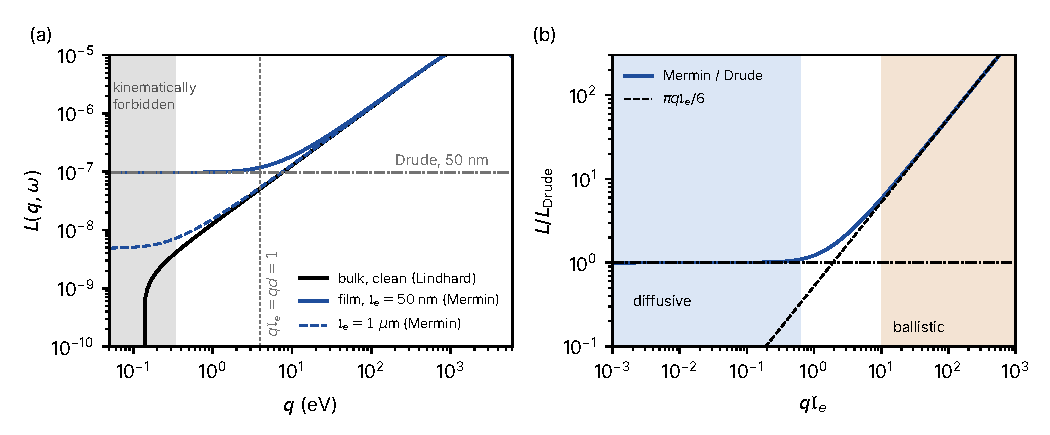
\includegraphics[width=\linewidth]{figures/ch15/fig15_2.pdf}
  \caption{Normal-state loss function of aluminum in a film and in the bulk. (a) $L(q,\omega)$ at $\omega = \SI{0.90}{meV}$ ($5\Delta_{\mathrm{BCS}}$ with the bulk gap) against the momentum transfer $q$, for a free-electron gas with $k_{\mathrm{F}} = \SI{1.75}{\angstrom^{-1}}$ and $v_{\mathrm{F}} = \num{6.75e-3}$. Curves: clean Lindhard function (black), Mermin function with mean free path $\mathfrak{l}_e = \SI{50}{nm}$ (blue, $\gamma_{\mathrm{rel}} = \SI{26.7}{meV}$) and $\mathfrak{l}_e = \SI{1}{\micro m}$ (blue dashed), and the Drude tail $\omega\gamma_{\mathrm{rel}}/\omega_p^2$ for \SI{50}{nm} (gray). Gray band: $q < \omega/v_{\mathrm{max}}$, out of reach of halo dark matter. Dotted vertical line: $q\mathfrak{l}_e = 1$, which for this film is also $qd_{\mathrm{film}} = 1$. (b) Ratio of the Mermin loss function to the Drude tail, against $q\mathfrak{l}_e$, for $q \ll k_{\mathrm{F}}$ (\cref{eq:15.3-mermin}) and $\omega/\gamma_{\mathrm{rel}} = 0.034$; dashed, the ballistic asymptote $\pi q\mathfrak{l}_e/6$. Shaded: within \SI{10}{\percent} of the diffusive limit (left) and of the ballistic limit (right), that is a ratio to the limit of at most 1.1.}
  \label{fig:15-film}
\end{figure}

\Cref{fig:15-film}a shows the consequence for aluminum. At the smallest momentum transfer that can deposit \SI{0.90}{meV}, $q = \omega/v_{\mathrm{max}} = \SI{0.34}{eV}$, the \SI{50}{nm} film has a loss function 24 times that of the clean crystal. The asymptotic $6/\pi q\mathfrak{l}_e$ is 22; the clean value lies below its own small-$\omega$ form there, since $\omega/qv_{\mathrm{F}} = 0.39$. The enhancement persists up to $q \approx 1/\mathfrak{l}_e = \SI{3.9}{eV}$, which is the largest momentum transfer of dark matter lighter than \SI{0.75}{keV}, and above that the two curves merge. A film with $\mathfrak{l}_e = \SI{1}{\micro m}$ lies between. Collisions in a film thus change the loss function for keV-mass dark matter, whereas at the momentum transfers of MeV-mass dark matter the film electrons are ballistic.

The plasmon width and the relaxation rate are different numbers. A Drude form fitted to the measured aluminum plasmon has $\omega_p = \SI{14.9}{eV}$ and a width of \SI{0.863}{eV}~\cite[Fig.~S1]{hochberg2021determining}, 32 times the relaxation rate of the \SI{50}{nm} film. The plasmon decays into electron--hole pairs by interband transitions and by collisions alike, while the tail at meV energies, by \cref{eq:15.3-limits}, is set by the dc resistivity, which measures momentum relaxation at the Fermi surface only. A tail extrapolated from the plasmon width overstates the loss function of the \SI{50}{nm} film at meV energies by that factor of 32.

The logarithms of the Lindhard function and of the BCS bubbles are taken on the retarded branch \cref{eq:C.8-branch}, which the limit of a vanishing width does not select by itself. The other branch suppresses the computed rate of an aluminum detector at low mass by up to seven orders of magnitude~\cite{hochberg2021determining}. A time-ordered bubble coincides with the retarded one at $T = 0$ only for $\omega > 0$, whereas a Kramers--Kronig integral and a sum rule need $\omega < 0$ as well.

\subsection{The superconducting film}\label{sec:15.3-sc}

On the kinematic edge of $y = \omega/\Delta_{\mathrm{BCS}} = 2.2$ the momentum transfer is $q = 2.2\,\Delta_{\mathrm{BCS}}/v_{\mathrm{max}} = \SI{0.15}{eV}$, whatever $v_{\mathrm{F}}$ is, so an aluminum film with $\mathfrak{l}_e = \SI{30}{nm}$ has $q\mathfrak{l}_e = 0.023$ there. Its electrons are diffusive on the scale of the probe, and the clean response of \cref{sec:15.1} does not apply. The conserving response with Born scattering by nonmagnetic impurities at $T = 0$ replaces it. In Nambu space the impurity potential couples through $\boldsymbol{\eta}$, the Nambu matrix of the density, so the Born self-energy is $\boldsymbol{\eta}\,\GF\,\boldsymbol{\eta}$ averaged over the Fermi surface. The same impurity ladder dresses the density vertex and the two pair vertices; with both, the response stays conserving (\cref{app:E.20}). Its normal state is the Mermin function \cref{eq:4.5-mermin} at the same relaxation rate $\gamma_{\mathrm{rel}} = v_{\mathrm{F}}/\mathfrak{l}_e$. \Cref{tab:15-edge} lists its edge values for \SI{1}{\micro m} and \SI{30}{nm}, divided by $\mathfrak{g}_{\mathrm{I}}$ times that normal state, and we use the same normalization for every number in this subsection.

At $y \ge 3$ the ratio hardly moves: it stays between 1.008 and 1.091 for every mean free path from \SI{100}{\micro m} down to \SI{30}{nm}. At $y \le 2.5$, however, it moves a great deal. At $y = 2.2$ it falls from 0.87 in the clean limit to 0.60 at $\mathfrak{l}_e = \SI{1}{\micro m}$, 0.38 at \SI{300}{nm} and 0.19 at \SI{30}{nm}, and at $y = 2.5$ from 1.00 to 0.57. The clean values hold to \SI{4}{\percent} down to $y = 2.2$ only for $\mathfrak{l}_e \ge \SI{10}{\micro m}$. In a film the suppression near the threshold therefore returns, now through the inductive response of the condensate.

The local limit of short mean free path shows why. When $q\mathfrak{l}_e \ll 1$ and $D_{\mathrm{diff}}q^2 \ll \Delta_{\mathrm{BCS}}$, neither an electron nor a pair resolves the spatial variation of the potential, and the film responds locally. The induced density then follows from the induced current by the continuity equation, longitudinal and transverse responses coincide (\cref{eq:4.4-ET}), and $\varepsilon = 1 + \ii\sigma_{\mathrm{cond}}(\omega)/\omega$ by \cref{eq:4.4-sigma}, in the superconducting state as in the normal one. The conductivity of a dirty superconductor is the Mattis--Bardeen conductivity, derived in \cref{sec:15.4-MB} and \cref{app:D.40}. At $T = 0$ its real part $\sigma_1/\sigma_n$ is the case-II pair-creation integral of \cref{eq:7.2-pairspec}, which is zero below $2\Delta_{\mathrm{BCS}}$ and rises continuously from zero above it. Its imaginary part $\sigma_2$ is the Kramers--Kronig partner of $\sigma_1$, and it contains the weight $(\pi^2/2)\Delta_{\mathrm{BCS}}\sigma_n$ missing from $\sigma_1$ below $2\Delta_{\mathrm{BCS}}$, which the condensate carries at $\omega = 0$. Since $|\varepsilon| \gg 1$, $-1/\varepsilon = \ii\omega/\sigma_{\mathrm{cond}}$, and
\begin{equation}
  L = \frac{\omega\,\sigma_1}{\sigma_1^2 + \sigma_2^2}, \qquad
  \frac{L_{\mathrm{s}}}{L_{\mathrm{n}}} = \frac{\sigma_n\,\sigma_1}{\sigma_1^2 + \sigma_2^2} \qquad (q\mathfrak{l}_e \ll 1,\ D_{\mathrm{diff}}q^2 \ll \Delta_{\mathrm{BCS}}) ,
  \label{eq:15.3-MB}
\end{equation}
with $L_{\mathrm{n}} = \omega/\sigma_n$ the Drude tail of \cref{eq:15.3-limits} and $L_{\mathrm{s}}$ the superconducting loss function. Near the threshold the ratio is small for two reasons. By continuity the density couples through the current, which is odd under time reversal, so the coherence factor is that of case~II, which vanishes at $2\Delta_{\mathrm{BCS}}$, rather than that of case~I with its step of $\pi/2$. And $\sigma_2$ exceeds $\sigma_1$ there, 0.757 against 0.139 times $\sigma_n$ at $y = 2.2$: the supercurrent of the condensate short-circuits the slow potential. Divided by $\mathfrak{g}_{\mathrm{I}}$, the normalization of \cref{tab:15-edge}, \cref{eq:15.3-MB} gives 0.157 at $y = 2.2$, 0.985 at $y = 3$, 1.094 at $y = 5$ and 1.023 at $y = 10$, against 0.187, 1.008, 1.091 and 1.021 in the \SI{30}{nm} column: \cref{eq:15.3-MB} is the end point of the table, and it needs only the measured conductivity of the film. At \SI{30}{nm} and $y = 2.2$ the conserving value still lies \SI{20}{\percent} above the local limit, although $D_{\mathrm{diff}}q^2 = 0.042\,\Delta_{\mathrm{BCS}}$ is already small there; the origin of that excess has not been established.

\subsection{Film thickness}\label{sec:15.3-sheet}

A film thicker than $1/q$ responds as the bulk. Its surfaces spread the momentum along the normal over a range $\sim 1/d_{\mathrm{film}}$, a relative correction of order $1/qd_{\mathrm{film}}$, and they carry surface plasmons near $\omega_p/\sqrt2 \approx \SI{11}{eV}$, far above the energies that dark matter deposits at these momenta. A film thinner than $1/q$ responds as a sheet. The external potential is then uniform across the thickness, and the film responds to its in-plane wavevector $\vect{q}_\parallel$ with the induced density $d_{\mathrm{film}}R(q_\parallel,\omega)\phi$ per area. This sheet of charge produces the potential $e^2/[(\varepsilon_a + \varepsilon_b)q_\parallel]\,\ee^{-q_\parallel|z|}$ per unit density, with $\varepsilon_a$ and $\varepsilon_b$ the dielectric constants of the media on the two sides. The two-dimensional Fourier transform of $e^2/4\pi r$ is $e^2/2q_\parallel$, and the image charges of the two half spaces replace the 2 by $\varepsilon_a + \varepsilon_b$. In the bulk the same density produces $e^2/q^2$. Therefore
\begin{equation}
  \varepsilon_{\mathrm{sh}}(q_\parallel,\omega) - 1 = \frac{q_\parallel d_{\mathrm{film}}}{\varepsilon_a + \varepsilon_b}\,\bigl[\varepsilon(q_\parallel,\omega) - 1\bigr] \qquad (qd_{\mathrm{film}} \ll 1) ,
  \label{eq:15.3-sheet}
\end{equation}
and the screening factor $1/|\varepsilon|^2$ in the structure factor $-2\Imag R/|\varepsilon|^2$ becomes $1/|\varepsilon_{\mathrm{sh}}|^2$, larger by $[(\varepsilon_a + \varepsilon_b)/q_\parallel d_{\mathrm{film}}]^2$ while both dielectric functions are large. For a slab in vacuum this is the leading term in $q_\parallel d_{\mathrm{film}}$ of the exact slab response of Lasenby and Prabhu~\cite[Eq.~(19)]{lasenby2022dark}, whose next term is of relative order $q_\parallel d_{\mathrm{film}}$. A thin metal film screens a long-wavelength potential far less than the bulk, because the field of its induced charge spreads outside it. The factor depends on the direction of $\vect{q}$ through $q_\parallel$, which makes the rate of a thin film directional. For this reason the QROCODILE analysis solves the electrostatic problem of a single \SI{2}{nm} WSi layer in vacuum with a Drude dielectric function; it finds the anisotropy strong at $q \sim \SI{1}{nm^{-1}}$ and already significant at $q \sim \SI{1}{keV}$ for energies above \SI{4}{eV}~\cite[supplement]{baudis2025first}. For the \SI{50}{nm} aluminum film $qd_{\mathrm{film}} = 1$ at $q = \SI{3.9}{eV}$, the same momentum at which $q\mathfrak{l}_e = 1$; for dark matter lighter than \SI{0.75}{keV} the film is a diffusive sheet at every momentum transfer. Stacks of sheets and the full slab need the response of a layered medium, which we do not treat here.

\begin{workedexample}{The Mermin loss function of a \SI{50}{nm} aluminum film}\label{we:15-film}
Take the free-electron gas of aluminum with $k_{\mathrm{F}} = \SI{3.45}{keV}$ and $v_{\mathrm{F}} = \num{6.75e-3}$, for which $k_{\mathrm{TF}} = \SI{4.05}{keV}$ and $\omega_p = \SI{15.78}{eV}$ by \cref{eq:4.4-TF}, and a mean free path $\mathfrak{l}_e = d_{\mathrm{film}} = \SI{50}{nm} = \SI{0.253}{eV^{-1}}$. Then $\gamma_{\mathrm{rel}} = v_{\mathrm{F}}/\mathfrak{l}_e = \SI{26.7}{meV}$ and $D_{\mathrm{diff}} = \SI{5.70e-4}{eV^{-1}}$ (\SI{337}{cm^2.s^{-1}}). Let a dark-matter particle deposit $\omega = 5\Delta_{\mathrm{BCS}} = \SI{0.90}{meV}$ with the bulk gap, at the smallest momentum transfer that allows it, $q = \omega/v_{\mathrm{max}} = \SI{0.340}{eV}$. Then $q\mathfrak{l}_e = 0.086$: the film is diffusive.

\emph{Mermin function.} With $qv_{\mathrm{F}} = \SI{2.29}{meV}$, $\mathfrak{w}_\gamma = 0.392 + 11.62\,\ii$, and \cref{eq:15.3-fL} gives $\mathfrak{f}_{\mathrm{L}} = (2.449 + 0.165\,\ii)\times10^{-3}$, within \SI{0.5}{\percent} of the tail $-1/3\mathfrak{w}_\gamma^2$. \Cref{eq:15.3-mermin} yields $\varepsilon_{\mathrm{Mer}} = (0.407 + 10.35\,\ii)\times10^{6}$, and the diffusion pole \cref{eq:15.3-diff}, with $D_{\mathrm{diff}}q^2 = \SI{0.066}{meV}$, is $(0.755 + 10.33\,\ii)\times10^{6}$: the imaginary parts agree, and the real parts differ at the order $\omega/\gamma_{\mathrm{rel}}$ that the pole drops. The loss function is $L_{\mathrm{Mer}} = \num{9.65e-8}$, \SI{0.2}{\percent} above the Drude tail $\omega\gamma_{\mathrm{rel}}/\omega_p^2 = \num{9.63e-8}$. The same number is $\varepsilon_0\omega\rho_{\mathrm{el}}$ with the residual resistivity \SI{0.80}{\micro\ohm.cm} of \cref{eq:15.3-rho}.

\emph{Comparisons.} The clean Lindhard function at the same point is $\varepsilon_{\mathrm{Lin}} = (1.19 + 0.88\,\ii)\times10^8$, with $L = \num{4.01e-9}$: the film absorbs 24 times more.

\emph{Superconducting film.} The film is dirty ($\mathfrak{l}_e/\xi_{\mathrm{coh}} = 0.021$), and $D_{\mathrm{diff}}q^2 = 0.37\,\Delta_{\mathrm{BCS}}$: \cref{eq:15.3-MB} applies roughly. At $y = 5$ it gives $L_{\mathrm{s}}/L_{\mathrm{n}} = 1.259$ and $L_{\mathrm{s}} = \num{1.21e-7}$. In the normalization of \cref{tab:15-edge} that is 1.094, and clean, intermediate and dirty films lie between 1.057 and 1.094 at this energy, within \SI{4}{\percent}; at $y = 2.2$ the clean value is 5.5 times the local limit.

\emph{Thickness.} Finally $qd_{\mathrm{film}} = 0.086$: the film is a sheet at this momentum, and in vacuum \cref{eq:15.3-sheet} reduces the screening by $q_\parallel d_{\mathrm{film}}/2$ for $\vect{q}$ in the plane, which multiplies the structure factor by $(2/0.086)^2 = 540$ to leading order in $q_\parallel d_{\mathrm{film}}$; the exact slab response of Lasenby and Prabhu gives 588. The bulk loss function computed here is the input to the sheet response, not the final answer.
\end{workedexample}

\subsection{Amorphous tungsten silicide}\label{sec:15.3-wsi}

Amorphous W$_x$Si$_{1-x}$ has no lattice, and its transport is measured, not computed. In \SI{5}{nm} films with $x = 0.75$--0.85 the sheet resistance, the resistance of a square of film, is 326--\SI{417}{\ohm}, a resistivity $\rho_{\mathrm{el}} = R_\square d_{\mathrm{film}}$ of 163--\SI{209}{\micro\ohm.cm}, 205 to 263 times that of the aluminum film of \cref{we:15-film}~\cite[Table~I]{zhang2016characteristics}. The magnetic field that destroys superconductivity rises below $T_c$ at a rate set by how fast the electrons diffuse, and its slope yields the diffusion constant 0.70--\SI{0.75}{cm^2.s^{-1}}. In a diffusive conductor the current is the diffusion current of the electrons that a field pushes off equilibrium, so the conductivity is $\sigma = e^2(2\mathcal{N}_{\mathrm{F}})D_{\mathrm{diff}}$, the Einstein relation. With the measured resistivity and diffusion constant of each film it gives the density of states $2\mathcal{N}_{\mathrm{F}} = $ (2.7--3.3)$\times10^{47}$\,m$^{-3}$\,J$^{-1}$, and at most \num{3.4e47}\,m$^{-3}$\,J$^{-1}$ for any combination of the measured values. The Ginzburg--Landau coherence length, the size of a pair measured near $T_c$, is 7.0--\SI{7.4}{nm}, and $T_c$ is 3.8--\SI{4.1}{K}. The \SI{2}{nm} W$_{0.45}$Si$_{0.55}$ layer of the QROCODILE detector has $T_c = \SI{1.73}{K}$~\cite{baudis2025first}, which gives $\Delta_{\mathrm{BCS}} = 1.764\,T_c = \SI{0.263}{meV}$.

The free-electron gas at $E_{\mathrm{F}} = \SI{7}{eV}$ has $k_{\mathrm{F}} = \SI{2.67}{keV}$, $v_{\mathrm{F}} = \num{5.23e-3}$ and $2\mathcal{N}_{\mathrm{F}} = \SI{1.13e47}{m^{-3}.J^{-1}}$. The density of states from the Einstein relation is 2.4--2.9 times larger: the gas does not describe these electrons, and the mean free path depends on which free-gas number is combined with the data. With the measured $D_{\mathrm{diff}}$ and \cref{eq:15.3-le}, $\mathfrak{l}_e = 3D_{\mathrm{diff}}/v_{\mathrm{F}} = 0.13$--\SI{0.14}{nm} and $k_{\mathrm{F}}\mathfrak{l}_e = 1.8$--1.9. With the measured resistivity and the free-gas $\omega_p = \SI{10.8}{eV}$, $\gamma_{\mathrm{rel}} = \varepsilon_0\omega_p^2\rho_{\mathrm{el}} = 2.5$--\SI{3.3}{eV}, $\mathfrak{l}_e = 0.32$--\SI{0.41}{nm} and $k_{\mathrm{F}}\mathfrak{l}_e = 4.3$--5.5. Either way $k_{\mathrm{F}}\mathfrak{l}_e = 2E_{\mathrm{F}}/\gamma_{\mathrm{rel}}$ is a few: the relaxation rate is comparable with the Fermi energy and the mean free path with the electron wavelength $2\pi/k_{\mathrm{F}} = \SI{0.46}{nm}$.

At the momentum transfers of MeV-mass dark matter, $q = 1$ to \SI{5}{keV}, this leaves no small parameter. There $q/k_{\mathrm{F}} = 0.37$--1.9 and $q\mathfrak{l}_e = 0.7$--3.4 with the shorter mean free path, while \cref{eq:15.3-fL} needs $q \ll k_{\mathrm{F}}$, the limits \cref{eq:15.3-limits} need $q\mathfrak{l}_e$ far from one, and a relaxation time itself needs $k_{\mathrm{F}}\mathfrak{l}_e \gg 1$, so that an electron has a momentum to relax. The Mermin function and its two limits are then all outside the conditions under which they were derived, and no correction factor to any of them can be quoted. At the pair-breaking edge the situation is the opposite. There $q = 2\Delta_{\mathrm{BCS}}/v_{\mathrm{max}} = \SI{0.20}{eV}$ and $q\mathfrak{l}_e \approx 10^{-4}$, and the diffusion pole \cref{eq:15.3-diff} holds for any conductor, since it needs only the continuity equation and Ohm's law with the Einstein relation. The normal-state loss function there is $\varepsilon_0\omega\rho_{\mathrm{el}} = (1.2$--$1.5)\times10^{-5}$ at $\omega = 2\Delta_{\mathrm{BCS}}$, fixed by the measured resistivity.

The superconducting part lies outside mean-field BCS. WSi is deep in the dirty limit, $\mathfrak{l}_e/\xi_{\mathrm{coh}} \approx 0.02$, where Anderson's theorem would keep the clean gap and \cref{eq:15.3-MB} would give the edge. But the theorem rests on disorder being weak: the density of states of the exact states, and the attraction between partners, change at relative order $1/k_{\mathrm{F}}\mathfrak{l}_e$, which is not small here. In addition, slow diffusion enhances the Coulomb repulsion between electrons, the Altshuler--Aronov effect. The enhanced repulsion competes with the pairing attraction and lowers $T_c$, the Finkel'stein mechanism~\cite[Sect.~III.2]{sacepe2020quantum}. BCS theory contains neither, and in strongly disordered films the gap also varies from place to place.

The rate of an amorphous film therefore needs the configurational average of the loss function over the amorphous structures, $\langle\Imag[-(\varepsilon^{-1})_{\vect{0}\vect{0}}]\rangle$, and the distribution of the local gap (\cref{app:E.20}). The average differs from the loss function of the averaged $\varepsilon$ at the order of the variance of $\varepsilon$. Both are open for amorphous WSi at momentum transfers of a keV.

\section{Absorption in superconductors and metals}\label{sec:15.4}

A dark photon of \SI{1}{meV} that is absorbed in aluminum gives up all of its energy but brings a momentum of only $m_\phi v \approx \SI{1}{\micro eV}$. To take up \SI{1}{meV}, an electron at the Fermi surface must change its momentum by at least $\omega/v_{\mathrm{F}} = \SI{0.15}{eV}$, a hundred thousand times more. A clean metal therefore cannot absorb the boson with one electron alone. A third body must take up the momentum: an impurity, which does so elastically, or a phonon, which carries off the momentum and part of the energy. \Cref{sec:10.7} expressed the rates of the dark photon and the axion-like particle through the optical conductivity $\sigma_1$ at the boson mass. In a metal below its interband threshold, about \SI{0.5}{eV} in aluminum~\cite[p.~4]{hochberg2016absorption}, that conductivity comes from the two third-body processes and from electron--electron collisions, a channel we name but do not size. Within a few gaps of the pair-breaking edge $2\Delta_{\mathrm{BCS}} = \SI{0.36}{meV}$ the superconducting state changes both third-body processes through the coherence factors of \cref{sec:7.2}: the phonon-assisted process carries the case-I factor and the impurity-assisted one the case-II factor. Both coherence factors follow from the structure of the current in the Nambu notation of \cref{sec:7.2}, and the phonon-assisted part reproduces the formula of Allen. In a clean singlet superconductor without spin--orbit coupling, the spin current, which absorbs the axion-like particle, breaks pairs without a third body.

\subsection{Impurity-assisted absorption}\label{sec:15.4-MB}

At $\vect{q} \to 0$ a dark photon, like a photon, couples to the total velocity $\op{\vect{V}}$ of the electrons, \cref{eq:6.5-HA}. In a metal below its interband threshold only the band that crosses the Fermi level contributes, and $\op{\vect{V}} = \sum_{\vect{k}\sigma}\vect{v}_{\vect{k}}\,c^\dagger_{\vect{k}\sigma}c_{\vect{k}\sigma}$ with the band velocity $\vect{v}_{\vect{k}} = \partial\xi_{\vect{k}}/\partial\vect{k}$. Time reversal makes $\xi_{-\vect{k}} = \xi_{\vect{k}}$, and therefore $\vect{v}_{-\vect{k}} = -\vect{v}_{\vect{k}}$. Relabeling $\vect{k} \to -\vect{k}$ in the spin-down term and writing the result with the Nambu spinors $\Psi_{\vect{k}}$ of \cref{eq:7.2-nambu} gives (\cref{app:D.40})
\begin{equation}
  \hat{\vect{e}}\cdot\op{\vect{V}} = \sum_{\vect{k}}(\hat{\vect{e}}\cdot\vect{v}_{\vect{k}})\,\Psi^\dagger_{\vect{k}}\Psi_{\vect{k}}
  = \sum_{\vect{k}}(\hat{\vect{e}}\cdot\vect{v}_{\vect{k}})\bigl(\gamma^\dagger_{\vect{k}1}\gamma_{\vect{k}1} - \gamma^\dagger_{\vect{k}2}\gamma_{\vect{k}2}\bigr) .
  \label{eq:15.4-Vnambu}
\end{equation}
The density is the matrix $\boldsymbol{\eta}$ in Nambu space; the uniform current is the unit matrix. The difference between the two matrices comes from the sign of the velocity under $\vect{k} \to -\vect{k}$, which the density, an even function of $\vect{k}$, does not have. The unit matrix commutes with $h_{\vect{k}}$, so the current commutes with $H_{\mathrm{MF}}$, and in the quasiparticle basis it only counts: $\gamma^\dagger_{\vect{k}1}$ carries the velocity $\vect{v}_{\vect{k}}$ of its electron $(\vect{k}\!\uparrow)$ and $\gamma^\dagger_{\vect{k}2}$ the velocity $\vect{v}_{-\vect{k}}$ of $(-\vect{k}\!\downarrow)$. The current creates no pairs. A clean BCS superconductor therefore absorbs nothing at $\vect{q} \to 0$ and $\omega > 0$, and the whole intraband weight of the f-sum rule lies at $\omega = 0$, as the supercurrent. The clean normal metal behaves the same way, with a Drude peak of zero width. This intraband weight is $(\pi/2)(\omega_p^{\mathrm{intra}})^2$, with the intraband plasma frequency
\begin{equation}
  (\omega_p^{\mathrm{intra}})^2 = 2e^2\,\mathcal{N}_{\mathrm{F}}\,\langle(\hat{\vect{e}}\cdot\vect{v})^2\rangle_{\mathrm{FS}} ,
  \label{eq:15.4-wp}
\end{equation}
where $\langle\dots\rangle_{\mathrm{FS}}$ is the average over the Fermi surface and the factor 2 counts the spins. For free electrons the intraband plasma frequency is $\omega_p$ of \cref{sec:4.3}, \SI{15.78}{eV} for the three valence electrons of aluminum; the computed bands of aluminum give \SI{12.29}{eV}~\cite[Table~IV]{savrasov1996electron}, which we use.

An impurity breaks the conservation of momentum, and with it the commutation of the current with $H_{\mathrm{MF}}$. The one-electron eigenstates $\alpha$ of the disordered metal have energies $\xi_\alpha$ and no definite momentum, but time reversal still pairs each with a partner $\bar\alpha$ of the same energy, and for nonmagnetic disorder the paired state is built from $(\alpha\!\uparrow, \bar\alpha\!\downarrow)$ with the same gap (\cref{sec:15.3}). The current acquires matrix elements $\langle\alpha|\hat{\vect{e}}\cdot\op{\vect{v}}|\beta\rangle$ between different states, and since it is odd under time reversal it is still the unit matrix in the Nambu space of $(\alpha, \bar\alpha)$. The pair-creation amplitude of the current then carries $u^{\mathrm{B}}_\alpha v^{\mathrm{B}}_\beta - v^{\mathrm{B}}_\alpha u^{\mathrm{B}}_\beta$, the case-II factor of \cref{eq:7.2-coh}, which vanishes for two quasiparticles at the gap edge (\cref{app:D.40}). In the dirty limit the relaxation rate $\gamma_{\mathrm{rel}} = v_{\mathrm{F}}/\mathfrak{l}_e$ far exceeds $\Delta_{\mathrm{BCS}}$ ($\mathfrak{l}_e \ll \xi_{\mathrm{coh}}$, \cref{sec:15.3}), and the squared matrix elements change only over energies of order $\gamma_{\mathrm{rel}}$. Over the few $\Delta_{\mathrm{BCS}}$ where the coherence factors matter, the squared matrix elements are constant, and $\xi_\alpha$ and $\xi_\beta$ are independent. The ratio of the superconducting to the normal absorption is then the case-II integral of \cref{eq:7.2-pairspec}:
\begin{keyresult}[Impurity-assisted absorption (Mattis--Bardeen)]
\begin{equation}
  \begin{gathered}
  \sigma_1^{\mathrm{MB}}(\omega) = \sigma_n(\omega)\,\mathfrak{g}_{\mathrm{II}}\Bigl(\frac{\omega}{\Delta_{\mathrm{BCS}}}\Bigr), \qquad
  \sigma_n(\omega) = \frac{\sigma_{\mathrm{dc}}\,\gamma_{\mathrm{rel}}^2}{\omega^2 + \gamma_{\mathrm{rel}}^2} , \\
  \mathfrak{g}_{\mathrm{II}}(y) = \Bigl(1 + \frac2y\Bigr)\mathrm{E}(k) - \frac4y\,\mathrm{K}(k) ,
  \end{gathered}
  \label{eq:15.4-MB}
\end{equation}
for $\omega \ge 2\Delta_{\mathrm{BCS}}$ and $\gamma_{\mathrm{rel}} \gg \Delta_{\mathrm{BCS}}$, with $\sigma_n$ the Drude conductivity of the normal metal, $\sigma_{\mathrm{dc}}$ its dc value, and $\mathrm{K}$, $\mathrm{E}$ the complete elliptic integrals of the modulus $k = (y - 2)/(y + 2)$ of \cref{eq:15.1-gI} (\cref{eq:D.40-g}).
\end{keyresult}
\noindent \Cref{eq:15.4-MB} is the absorption of light by a superconductor that Mattis and Bardeen found~\cite{mattis1958theory}; \cref{sec:7.2} met its zero-temperature ratio as the case-II pair-creation spectrum. The function $\mathfrak{g}_{\mathrm{II}}$ starts from zero at the edge, is 0.67 at $4\Delta_{\mathrm{BCS}}$ and comes within \SI{10}{\percent} of one at $8.1\,\Delta_{\mathrm{BCS}}$; its case-I partner $\mathfrak{g}_{\mathrm{I}}$ of \cref{sec:15.1} has the same closed form with $4/(y + 2)$ in place of $4/y$. No ladder of the pair field corrects \cref{eq:15.4-MB}. In the conserving response \cref{eq:7.2-Rc} the current would couple to the amplitude and phase channels through bubbles that pair one odd factor $\vect{v}$ with an even pair vertex, and these bubbles vanish. The bubble of independent quasiparticles in the exact impurity states is already the conserving response at $\vect{q} \to 0$, and through the continuity equation it is the long-wavelength limit of the density response of \cref{sec:15.1}.

Impurity-assisted absorption is large in a film. The \SI{50}{nm} aluminum film of \cref{we:15-film}, with $\mathfrak{l}_e = \SI{50}{nm}$, has $\gamma_{\mathrm{rel}} = \SI{26.7}{meV}$, 148 gaps, and with the free-electron plasma frequency its dc conductivity is $\sigma_{\mathrm{dc}} = \omega_p^2/\gamma_{\mathrm{rel}} = \SI{9.35e3}{eV}$, a residual resistivity of \SI{0.80}{\micro\ohm.cm}. At \SI{1}{meV} the paired film absorbs with $\sigma_1^{\mathrm{MB}} = \SI{7.56e3}{eV}$, $1.4\times10^6$ times the phonon-assisted value derived next. Intrinsic absorption dominates only in a pure sample, as Hochberg, Lin and Zurek assumed~\cite{hochberg2016absorption}, and in a film the rate follows the residual resistivity of the sample, not a property of aluminum.

\subsection{Phonon-assisted absorption}\label{sec:15.4-holstein}

In a pure crystal the third body is a phonon. The absorption is then of second order, with one current vertex and one electron--phonon vertex, as for phonon-assisted absorption across the gap of silicon (\cref{sec:6.5}), and the phonon carries the momentum that the electrons need. At \SI{1}{meV} in aluminum the phonon has at most $\omega - 2\Delta_{\mathrm{BCS}} = \SI{0.64}{meV}$. With the sound speeds along [100] from the zero-temperature elastic constants, $c_{\mathrm{LA}} = \SI{6.47}{km.s^{-1}}$ and $c_{\mathrm{TA}} = (C_{44}/\rho)^{1/2} = \SI{3.40}{km.s^{-1}}$ for $C_{44} = \SI{31.6}{GPa}$~\cite[Table~2]{malica2020quasi} and $\rho = \SI{2.73}{g.cm^{-3}}$, that is a momentum of at most 29.7 or \SI{56.4}{eV}. The smaller value is two hundred times the \SI{0.15}{eV} that the electrons need, and the larger is 61 times less than $k_{\mathrm{F}} = \SI{3.45}{keV}$, so only long-wavelength acoustic phonons take part near the edge. In a superconductor the question is which coherence factor the final pair carries, and the Nambu form \cref{eq:15.4-Vnambu} answers it exactly.

Take the electron--phonon Hamiltonian \cref{eq:A.6-Hep} restricted to the band at the Fermi level, with the vertex $g_\nu(\vect{k},\vect{Q})$, and the final states with one quasiparticle in $(\vect{k}+\vect{Q}\!\uparrow)$, one in $(-\vect{k}\!\downarrow)$ and an emitted phonon $(-\vect{Q},\nu)$. The second-order amplitude has the two time orderings of \cref{eq:13.2-T}, with the current in place of the density. The current is diagonal in the quasiparticle basis, so every intermediate state reached by the current is the state it acted on. The sum over intermediate states collapses, and the amplitude is the matrix element of the phonon vertex times the change of the current eigenvalue, $J_f - J_i$, divided by $-\omega$ (\cref{eq:D.40-T}). The ground state carries no current, and by \cref{eq:15.4-Vnambu} the final pair carries $\hat{\vect{e}}\cdot(\vect{v}_{\vect{k}+\vect{Q}} - \vect{v}_{\vect{k}})$. The phonon vertex creates the pair through its spin-up and spin-down terms, as the density does in \cref{eq:7.2-coh}. With the phase convention in which time reversal gives $g_\nu(-\vect{k}-\vect{Q},\vect{Q}) = g_\nu(\vect{k},\vect{Q})$,
\begin{keyresult}[Phonon-assisted amplitude in a superconductor]
\begin{equation}
  T_{fi} = -\frac{\hat{\vect{e}}\cdot(\vect{v}_{\vect{k}+\vect{Q}} - \vect{v}_{\vect{k}})}{\omega}\,\frac{1}{\sqrt N}\,g_\nu(\vect{k},\vect{Q})\,\bigl(u^{\mathrm{B}}_{\vect{k}+\vect{Q}}v^{\mathrm{B}}_{\vect{k}} + v^{\mathrm{B}}_{\vect{k}+\vect{Q}}u^{\mathrm{B}}_{\vect{k}}\bigr) ,
  \label{eq:15.4-T}
\end{equation}
for $|f\rangle = \gamma^\dagger_{\vect{k}+\vect{Q},1}\gamma^\dagger_{\vect{k}2}b^\dagger_{-\vect{Q}\nu}|\mathrm{BCS}\rangle$ at $T = 0$, with $\omega = E_{\vect{k}+\vect{Q}} + E_{\vect{k}} + \omega_{\vect{Q}\nu}$ and $N$ the number of unit cells.
\end{keyresult}
\noindent No intermediate state needs to be far from the energy shell. The only input is that the current commutes with the mean-field Hamiltonian, and the result holds for any $\omega$ and any phonon energy. The current supplies only the velocity difference, the factor that suppresses forward scattering. The pair itself is created by the phonon, through a vertex even under time reversal, and so it carries the case-I factor of the density. Phonon-assisted absorption has the coherence factor of the density, impurity-assisted absorption that of the current. The same steps with the density in place of the current give zero, because the eigenvalue of the density at $\vect{q} = 0$ is the conserved electron number, as in \cref{eq:13.2-q0}.

The conductivity follows from the absorbed power as in \cref{sec:6.5},
\begin{equation*}
  \sigma_1 = \frac{\pi e^2}{\omega\Vol}\sum_f|T_{fi}|^2\,\delta(E_f - E_i - \omega) .
\end{equation*}
The band velocity and the vertex change across the Fermi surface on scales of eV, whereas $\xi_{\vect{k}}$ and $\xi_{\vect{k}+\vect{Q}}$ range only over $\omega$. The sum over $\vect{k}$ and $\vect{Q}$ therefore splits into an average over the Fermi surface and independent integrals over the two energies. The integrals give the pair spectrum $2x\,\mathfrak{g}_{\mathrm{I}}(x/\Delta_{\mathrm{BCS}})$ at the pair energy $x = \omega - \omega_{\vect{Q}\nu}$, the case-I integral of \cref{eq:7.2-pairspec}. The average defines the transport Eliashberg function,
\begin{equation}
  \alpha^2F_{\mathrm{tr}}(\omega) = \frac{1}{2\langle(\hat{\vect{e}}\cdot\vect{v})^2\rangle_{\mathrm{FS}}\,\mathcal{N}_{\mathrm{F}}\Omega\,N^2}\sum_{\vect{k}\vect{Q}\nu}|g_\nu(\vect{k},\vect{Q})|^2\bigl[\hat{\vect{e}}\cdot(\vect{v}_{\vect{k}+\vect{Q}} - \vect{v}_{\vect{k}})\bigr]^2\delta(\xi_{\vect{k}})\,\delta(\xi_{\vect{k}+\vect{Q}})\,\delta(\omega - \omega_{\vect{Q}\nu}) ,
  \label{eq:15.4-a2Ftr}
\end{equation}
with $\Omega$ the volume of the unit cell, so that $\Vol = N\Omega$. This transport function is the Eliashberg function of \cref{eq:6.4-a2F} with each pair of Fermi-surface points weighted by the change of the velocity. For a spherical Fermi surface in a cubic crystal the weight averages to $\langle[\hat{\vect{e}}\cdot(\vect{v}' - \vect{v})]^2\rangle = 2(1 - \cos\theta_{\vect{k}\vect{k}+\vect{Q}})\langle(\hat{\vect{e}}\cdot\vect{v})^2\rangle_{\mathrm{FS}}$, and with the factor $\frac12$ of the definition the weight is $1 - \cos\theta_{\vect{k}\vect{k}+\vect{Q}}$, which removes forward scattering. The transport coupling constant is $\lambda_{\mathrm{tr}} = 2\int\dd\omega\,\alpha^2F_{\mathrm{tr}}(\omega)/\omega$. Inserting \cref{eq:15.4-wp} gives (\cref{app:D.40})
\begin{keyresult}[Phonon-assisted (Holstein) absorption]
\begin{equation}
  \begin{gathered}
  \sigma_1^{\mathrm{S}}(\omega) = \frac{(\omega_p^{\mathrm{intra}})^2}{\omega^2}\,\frac{2\pi}{\omega}\int_0^{\omega - 2\Delta_{\mathrm{BCS}}}\dd\omega'\,\alpha^2F_{\mathrm{tr}}(\omega')\,(\omega - \omega')\,\mathfrak{g}_{\mathrm{I}}\Bigl(\frac{\omega - \omega'}{\Delta_{\mathrm{BCS}}}\Bigr) , \\
  \sigma_1^{\mathrm{N}}(\omega) = \frac{(\omega_p^{\mathrm{intra}})^2}{\omega^2}\,\gamma_{\mathrm{H}}(\omega), \qquad
  \gamma_{\mathrm{H}}(\omega) = \frac{2\pi}{\omega}\int_0^{\omega}\dd\omega'\,(\omega - \omega')\,\alpha^2F_{\mathrm{tr}}(\omega') ,
  \end{gathered}
  \label{eq:15.4-holstein}
\end{equation}
for the superconductor and the normal metal at $T = 0$, $\omega$ below the interband threshold and above the impurity rate.
\end{keyresult}
\noindent The normal-metal form is Allen's formula for the phonon-assisted optical conductivity~\cite{allen1971electron}, as quoted by Hochberg, Lin and Zurek~\cite[Eqs.~(13), (16)]{hochberg2016absorption}: a Drude conductivity at $\omega \gg \gamma_{\mathrm{H}}$ with the frequency-dependent scattering rate $\gamma_{\mathrm{H}}(\omega)$ of an electron that absorbs $\omega$ and emits a phonon. The superconducting form, with its case-I factor and the bound $\omega' \le \omega - 2\Delta_{\mathrm{BCS}}$, is also Allen's~\cite[Eq.~(17)]{hochberg2016absorption}, and it holds for intermediate states on shell as well. Two of its hypotheses can be sized. The pair created by the phonon is not dressed by the ladder of \cref{eq:7.2-Rc}. The ladder correction is of relative order $(\Delta_{\mathrm{BCS}}/v_{\mathrm{F}}Q)^2$ at the phonon momentum $Q$ (\cref{sec:7.2}); averaged over the integrand of \cref{eq:15.4-holstein} with the $\omega'^4$ law below, it is $4\times10^{-4}$ at $\omega = 2.2\,\Delta_{\mathrm{BCS}}$ ($2.6\times10^{-4}$ for the most energetic phonon) and $1.4\times10^{-6}$ at \SI{1}{meV}. At millikelvin temperatures there are no thermal phonons to absorb, and thermal quasiparticles are suppressed by $\ee^{-\Delta_{\mathrm{BCS}}/T}$ (\cref{sec:7.2}).

The dark-matter literature evaluates \cref{eq:15.4-holstein} with a Debye transport function, $\alpha^2F_{\mathrm{tr}}(\omega') = 2\lambda_{\mathrm{tr}}\omega'^4/\omega_{\mathrm{D}}^4$ below $\omega_{\mathrm{D}}$, which carries the coupling $\lambda_{\mathrm{tr}}$. The fourth power is that of long-wavelength longitudinal phonons: $\alpha^2F$ grows as $\omega'^2$ (\cref{sec:6.4}), and the transport weight $1 - \cos\theta \propto Q^2$ adds two more powers. The rate is then $\gamma_{\mathrm{H}} = (2\pi/15)\lambda_{\mathrm{tr}}\omega^5/\omega_{\mathrm{D}}^4$ below $\omega_{\mathrm{D}}$, and above it $\gamma_{\mathrm{H}} = (4\pi/5)\lambda_{\mathrm{tr}}\omega_{\mathrm{D}}(1 - 5\omega_{\mathrm{D}}/6\omega)$, the result of Ref.~\cite[Eq.~(16)]{hochberg2016absorption}, and the ratio of the two lines of \cref{eq:15.4-holstein} is their Eq.~(17) (\cref{app:D.40}). Below $\omega_{\mathrm{D}}$ that ratio depends only on the power law, not on $\lambda_{\mathrm{tr}}$ or $\omega_{\mathrm{D}}$. For aluminum we take $\omega_{\mathrm{D}} = \SI{37}{meV}$~\cite{hochberg2016absorption} and $\lambda_{\mathrm{tr}} = 0.39$, the value that Savrasov and Savrasov extract from the measured resistivity with their computed plasma frequency~\cite[Table~IV]{savrasov1996electron}; their linear-response calculation gives 0.37. \Cref{lim:15.4a} compares the superconducting rate with the normal-metal formula.

\begin{limitbox}[Phonon-assisted absorption: the normal-metal limit][lim:15.4a]
Phonon-assisted absorption of a superconductor, \cref{eq:15.4-holstein} with $\alpha^2F_{\mathrm{tr}} = 2\lambda_{\mathrm{tr}}\omega'^4/\omega_{\mathrm{D}}^4$~\cite[Eqs.~(13), (16), (17)]{hochberg2016absorption}, following Allen~\cite{allen1971electron} as quoted there; for $\omega \gg \Delta_{\mathrm{BCS}}$ it becomes the normal-metal formula $\sigma_1^{\mathrm{N}} = (\omega_p^{\mathrm{intra}})^2\gamma_{\mathrm{H}}/\omega^2$.
\par\smallskip
{\centering
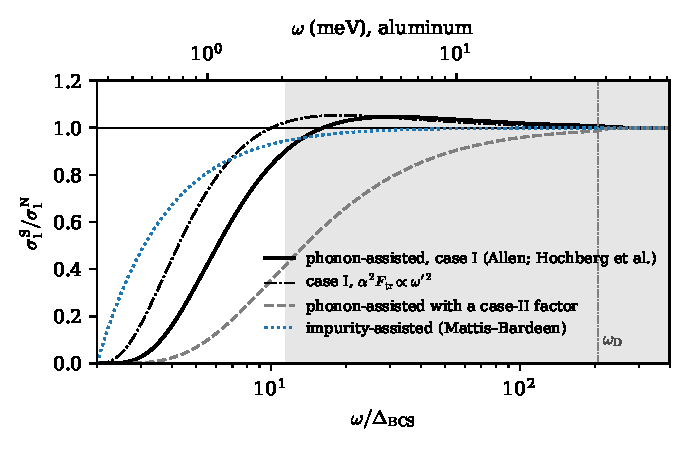
\includegraphics[width=0.85\linewidth]{figures/ch15/limit15_4a.pdf}
\captionof{figure}{Phonon-assisted conductivity of a superconductor over that of the normal metal, $\sigma_1^{\mathrm{S}}/\sigma_1^{\mathrm{N}}$, against $\omega/\Delta_{\mathrm{BCS}}$ (top axis: $\omega$ for aluminum, $\Delta_{\mathrm{BCS}} = \SI{0.18}{meV}$), at $T = 0$. Black: \cref{eq:15.4-holstein} with the case-I factor and the Debye law $\alpha^2F_{\mathrm{tr}} \propto \omega'^4$, which is the ratio of Hochberg, Lin and Zurek and, below $\omega_{\mathrm{D}}$ (dash-dotted vertical line, \SI{37}{meV}), independent of $\lambda_{\mathrm{tr}}$ and $\omega_{\mathrm{D}}$; dash-dotted: the same with the softer law $\alpha^2F_{\mathrm{tr}} \propto \omega'^2$, a test of the shape. Thin line at one: the normal-metal formula of Allen. Dashed: the phonon-assisted integral with the case-II factor in place of the case-I factor, for comparison. Dotted: impurity-assisted absorption in the dirty limit, $\mathfrak{g}_{\mathrm{II}}(\omega/\Delta_{\mathrm{BCS}})$, \cref{eq:15.4-MB}. Gray: the case-I result within \SI{10}{\percent} of the normal-metal formula, $\omega \ge 11.4\,\Delta_{\mathrm{BCS}}$ (\SI{2.05}{meV}).}\label{fig:15-limit-holstein}
\par}
\smallskip
Below $11.4\,\Delta_{\mathrm{BCS}}$ the normal-metal formula overstates the rate, by a factor of 2.4 at \SI{1}{meV} and without bound toward the edge, where the superconducting rate falls as $(\omega - 2\Delta_{\mathrm{BCS}})^5$; there the result also depends on the shape of $\alpha^2F_{\mathrm{tr}}$ below a few meV (0.42 or 0.73 of the normal value at \SI{1}{meV} for the two laws).
\end{limitbox}

The gap removes the absorption near the edge for a reason of phase space, not of coherence. The case-I factor is largest at the edge, where $\mathfrak{g}_{\mathrm{I}} = \pi/2$, but a phonon of energy $\omega'$ is available only up to $\omega - 2\Delta_{\mathrm{BCS}}$. Since $\alpha^2F_{\mathrm{tr}}$ grows as $\omega'^4$, the gap removes the most energetic phonons, which carry most of the weight. Above $16\,\Delta_{\mathrm{BCS}}$ the pile-up of the case-I factor dominates and the superconductor absorbs slightly more than the normal metal, by at most \SI{4.7}{\percent}, at $31\,\Delta_{\mathrm{BCS}}$. Had the pair carried the case-II factor of impurity-assisted absorption, the rate would reach \SI{90}{\percent} of the normal value only at $54\,\Delta_{\mathrm{BCS}}$. \Cref{fig:15-absorption}a shows the two processes on an absolute scale. The phonon-assisted conductivity of the normal metal grows as $\omega^3$ up to $\omega_{\mathrm{D}}$ and falls as $\omega^{-2}$ above. The impurity-assisted conductivity of the \SI{50}{nm} film, however, is flat up to $\gamma_{\mathrm{rel}}$ and stays above the phonon-assisted conductivity at every energy of the figure, by a factor of 1.6 at \SI{0.1}{eV} and 1.3 at \SI{0.3}{eV}.

\begin{figure}[tbp]
  \centering
  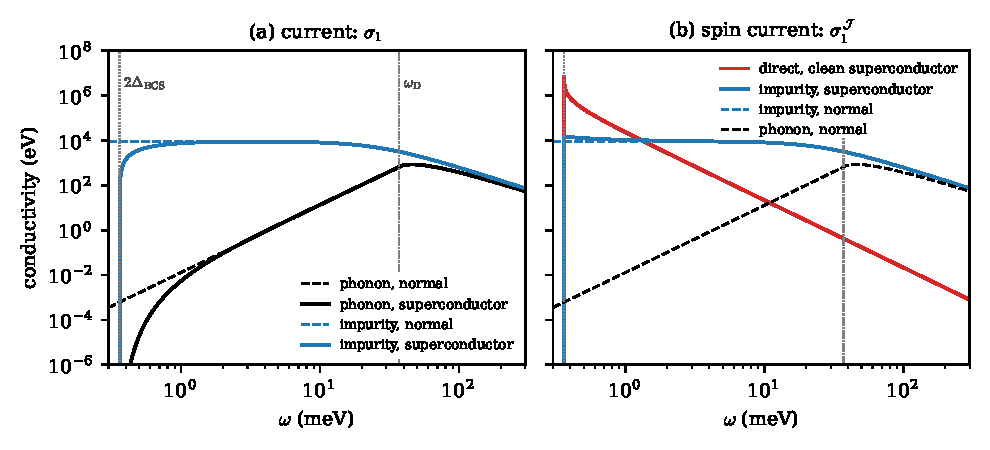
\includegraphics[width=\linewidth]{figures/ch15/fig15_3.pdf}
  \caption{Absorption of a uniform field by aluminum at $T = 0$, against the boson energy $\omega$, with $\Delta_{\mathrm{BCS}} = \SI{0.18}{meV}$ (dotted vertical line at $2\Delta_{\mathrm{BCS}}$) and the computed intraband plasma frequency \SI{12.29}{eV}. (a) Optical conductivity $\sigma_1$, which sets the rates of the dark photon. Black: phonon-assisted, \cref{eq:15.4-holstein}, in the normal metal (dashed) and the superconductor (solid), with the Debye transport function, $\lambda_{\mathrm{tr}} = 0.39$ and $\omega_{\mathrm{D}} = \SI{37}{meV}$ (dash-dotted vertical line). Blue: impurity-assisted, the Drude conductivity of the normal metal (dashed) and the Mattis--Bardeen conductivity of the superconductor (solid), \cref{eq:15.4-MB}, for the \SI{50}{nm} film of \cref{we:15-film} (mean free path \SI{50}{nm}, $\gamma_{\mathrm{rel}} = \SI{26.7}{meV}$, free-electron plasma frequency \SI{15.78}{eV} in its Drude conductivity). (b) Spin-current conductivity $\sigma_1^{\mathcal{J}}$, which sets the rate of the axion-like particle, normalized to equal $\sigma_1$ in the normal metal. Red: direct pair breaking in the clean superconductor, \cref{eq:15.4-sJ} with the quasiparticle factor $1/(1 + \lambda_{\mathrm{ep}}) = 0.70$. Blue: impurity-assisted, with the case-I factor in the superconductor (solid) and the Drude form in the normal metal (dashed), same mean free path. Black dashed: the phonon-assisted conductivity of the normal metal, for reference. Interband absorption, above about \SI{0.5}{eV}, is not included.}
  \label{fig:15-absorption}
\end{figure}

\begin{workedexample}{The Holstein onset in aluminum}\label{we:15-holstein}
A dark photon of $m_\phi = \SI{1}{meV}$, $5.56\,\Delta_{\mathrm{BCS}}$, is absorbed by pure aluminum with one phonon. The Debye form gives the normal-metal scattering rate $\gamma_{\mathrm{H}} = (2\pi/15)\lambda_{\mathrm{tr}}\omega^5/\omega_{\mathrm{D}}^4 = \SI{8.72e-11}{eV}$, and with $\omega_p^{\mathrm{intra}} = \SI{12.29}{eV}$ the normal-metal conductivity is $\sigma_1^{\mathrm{N}} = (\omega_p^{\mathrm{intra}})^2\gamma_{\mathrm{H}}/\omega^2 = \SI{0.0132}{eV}$. The superconductor has $\sigma_1^{\mathrm{S}}/\sigma_1^{\mathrm{N}} = 0.421$, so $\sigma_1^{\mathrm{S}} = \SI{5.54e-3}{eV}$.

Close to the edge the integral of \cref{eq:15.4-holstein} simplifies. For $\omega - 2\Delta_{\mathrm{BCS}} \ll \Delta_{\mathrm{BCS}}$ the pair energy $\omega - \omega'$ stays near $2\Delta_{\mathrm{BCS}}$ and $\mathfrak{g}_{\mathrm{I}}$ near $\pi/2$, and
\begin{equation*}
  \sigma_1^{\mathrm{S}} \simeq \frac{(\omega_p^{\mathrm{intra}})^2}{\omega^2}\,\frac{2\pi}{\omega}\,\frac{2\lambda_{\mathrm{tr}}}{\omega_{\mathrm{D}}^4}\,\frac{\pi}{2}\,2\Delta_{\mathrm{BCS}}\,\frac{(\omega - 2\Delta_{\mathrm{BCS}})^5}{5} .
\end{equation*}
At $\omega = 2.05$ and $2.5\,\Delta_{\mathrm{BCS}}$ this approximation is within 0.2 and \SI{2.1}{\percent} of the full integral. At $2.2\,\Delta_{\mathrm{BCS}}$ the superconductor absorbs with $\sigma_1^{\mathrm{S}} = \SI{4.4e-8}{eV}$, against $\SI{8.2e-4}{eV}$ for the normal metal: in practice the onset lies above $2\Delta_{\mathrm{BCS}}$.

The rate needs the loss function, $L = \varepsilon_2/|\varepsilon|^2$ in \cref{eq:10.7-dp}. At \SI{1}{meV} the condensate dominates $\varepsilon$: in the clean superconductor at $T = 0$ the imaginary conductivity is $\sigma_2 = (\omega_p^{\mathrm{intra}})^2/\omega$, and $\varepsilon_1 = 1 - \sigma_2/\omega = -1.51\times10^8$. The in-medium factor $1/|\varepsilon|^2$ is $4.4\times10^{-17}$, and $L = \sigma_1^{\mathrm{S}}\omega^3/(\omega_p^{\mathrm{intra}})^4 = 2.43\times10^{-16}$. With $\rho_\chi = \SI{0.3}{GeV.cm^{-3}}$ and $\rho_T = \SI{2.70}{g.cm^{-3}}$, \cref{eq:10.7-dp} gives $1.29\times10^{18}\,\zeta^2$ events per kilogram-year, and three events need $\zeta = 1.5\times10^{-9}$. The normal-metal formula would claim $9.9\times10^{-10}$. In the \SI{50}{nm} film of \cref{we:15-film} the impurity-assisted conductivity at the same mass is $1.4\times10^6$ times larger, and the rate with it.
\end{workedexample}

\subsection{Spin-current absorption}\label{sec:15.4-spin}

The axion-like particle couples through $(\partial_t\phi)\mathcal{J}^{\alpha\alpha}_e$. Here $\mathcal{J}_e = \sum_\alpha\mathcal{J}^{\alpha\alpha}_e$ is the spin current of the electrons traced over its two indices, a scalar like $\boldsymbol{\sigma}\cdot\vect{v}$ (\cref{sec:10.7-alp}). \Cref{sec:10.7-alp} reduced the rate of the axion-like particle to the optical conductivity through the spin trace $S_{\mathcal{J}\mathcal{J}} = \frac34S_{jj}$, valid for independent electrons without spin--orbit coupling. In a superconductor we keep the response of the spin current itself and define its conductivity by
\begin{equation}
  \sigma_1^{\mathcal{J}}(\omega) = \frac{2e^2}{3\omega}\,S_{\mathcal{J}\mathcal{J}}(0,\omega) ,
  \label{eq:15.4-sJdef}
\end{equation}
so that \cref{eq:10.7-alp} holds with $\sigma_1^{\mathcal{J}}$ in place of $\sigma_1$, and $\sigma_1^{\mathcal{J}} = \sigma_1$ in the normal metal. The component of the spin current with the spin and the velocity both along $\hat{\vect{z}}$ is $\mathcal{J}^{zz}_e = \frac12\sum_{\vect{k}}v^z_{\vect{k}}(c^\dagger_{\vect{k}\uparrow}c_{\vect{k}\uparrow} - c^\dagger_{\vect{k}\downarrow}c_{\vect{k}\downarrow})$. The relabeling that turned the current into the unit matrix now meets a second sign, that of the spin, and the two cancel: $\mathcal{J}^{zz}_e = \frac12\sum_{\vect{k}}v^z_{\vect{k}}\Psi^\dagger_{\vect{k}}\boldsymbol{\eta}\Psi_{\vect{k}}$, with the matrix of the density. That matrix does not commute with $h_{\vect{k}}$. In the quasiparticle basis (\cref{eq:D.40-bogo}) the spin current contains the term $\frac12v^z_{\vect{k}}(\Delta_{\mathrm{BCS}}/E_{\vect{k}})\gamma^\dagger_{\vect{k}1}\gamma^\dagger_{\vect{k}2}$, which creates a pair of total momentum zero and energy $2E_{\vect{k}}$. A uniform charge current moves both electrons of a pair $(\vect{k}\!\uparrow, -\vect{k}\!\downarrow)$ in the same direction and only boosts the condensate. A spin current drives the spin-up and spin-down electrons in opposite directions, pulls the two members of each pair apart, and breaks pairs.

In a clean superconductor this pair breaking needs no third body. Without spin--orbit coupling the three components $\mathcal{J}^{\alpha\alpha}_e$ contribute equally and do not interfere, and the golden rule with the amplitude above gives (\cref{app:D.40})
\begin{keyresult}[Spin-current absorption in a clean superconductor]
\begin{equation}
  \sigma_1^{\mathcal{J}}(\omega) = \frac{2\pi(\omega_p^{\mathrm{intra}})^2\,\Delta_{\mathrm{BCS}}^2}{\omega^2\,(\omega^2 - 4\Delta_{\mathrm{BCS}}^2)^{1/2}}\,\Theta(\omega - 2\Delta_{\mathrm{BCS}}) ,
  \label{eq:15.4-sJ}
\end{equation}
at $T = 0$, without spin--orbit coupling, for a mean free path long compared with the size of a pair; its integral over $\omega$ is $(\pi/2)(\omega_p^{\mathrm{intra}})^2$.
\end{keyresult}
\noindent In the clean normal metal the spin current commutes with the one-body band Hamiltonian, but not with the interactions. A two-body force enters with the weight of the spin difference, $[p^z_1\sigma^z_1 + p^z_2\sigma^z_2, V(\vect{r}_1 - \vect{r}_2)] = -\ii\,(\partial_zV)(\sigma^z_1 - \sigma^z_2)$, which vanishes for parallel spins only. Galilean invariance protects the charge current, whose internal forces cancel in pairs, but not the spin current. Electron--electron collisions (spin Coulomb drag) and normal phonon processes relax it, and its normal-state weight forms a narrow Drude peak rather than a delta function at $\omega = 0$. With a collision rate $\beta\omega^2$ and $\beta = 0.03$ to \SI{0.3}{eV^{-1}}, an estimate of the Fermi-liquid scale, the normal metal at $T \to 0$ absorbs at \SI{0.72}{meV} with $\sigma_1^{\mathcal{J}} \approx 5$ to \SI{45}{eV}, against the phonon-assisted $\sigma_1^{\mathrm{N}} = \SI{4.9e-3}{eV}$; the superconducting direct term is $1.5\times10^3$ to $1.5\times10^4$ times larger still. Pairing keeps the charge-current weight at zero frequency, as the supercurrent, and moves the spin-current weight above $2\Delta_{\mathrm{BCS}}$: \SI{87}{\percent} of it lies below $4\Delta_{\mathrm{BCS}}$ and \SI{99.5}{\percent} below $20\Delta_{\mathrm{BCS}}$. The total weight is fixed beyond mean field: for any Hamiltonian that does not depend on spin, the spin current is the time derivative of the spin dipole, and its integrated absorption obeys an exact sum rule (\cref{app:D.40}). The total weight, interband absorption included, equals the total weight of the charge current, $(\pi/2)\omega_p^2$ with the free-electron $\omega_p$; for the conduction band alone, a one-band Hamiltonian with spin-independent interactions, it is $(\pi/2)(\omega_p^{\mathrm{intra}})^2$ exactly. The part near $2\Delta_{\mathrm{BCS}}$ is the coherent quasiparticle weight $(\pi/2)(\omega_p^{\mathrm{intra}})^2(1 + F_1^a/3)/(1 + \lambda_{\mathrm{ep}})$, with the Landau parameter $F_1^a$ of the quasiparticle spin current and the residue $1/(1 + \lambda_{\mathrm{ep}})$ of \cref{eq:6.4-mass}; the rest of the spin-current weight lies near $\omega_{\mathrm{D}}$, like the Holstein band of the charge current, and at the scale of the Fermi energy. The sum rule therefore requires \cref{eq:15.4-sJ} near the edge to carry the factor $(1 + F_1^a/3)/(1 + \lambda_{\mathrm{ep}})$, which is 0.70 for $F_1^a = 0$ and the measured $\lambda_{\mathrm{ep}} = 0.43$ of \cref{sec:6.4}. The bare BCS bubble is conserving in the spin channel, and a singlet superconductor has zero spin stiffness, as its Pauli susceptibility vanishes, so the weight cannot lie at $\omega = 0$ (\cref{app:D.40}). In a dirty film the matrix elements of $\mathcal{J}_e$ between impurity states replace the direct term. Since the spin current is even under time reversal, the steps of \cref{eq:15.4-MB} give $\sigma_n\mathfrak{g}_{\mathrm{I}}(\omega/\Delta_{\mathrm{BCS}})$, with the factor of the density, which jumps to $\pi/2$ at the edge. That form conserves the normal-state weight exactly for a flat $\sigma_n$, since $\int_2^\infty\dd y\,[\mathfrak{g}_{\mathrm{I}}(y) - 1] = 2$: the weight above $2\Delta_{\mathrm{BCS}}$ replaces the weight below. For the Drude $\sigma_n$ of the \SI{50}{nm} film the balance holds to \SI{0.05}{\percent}, the residue coming from the Drude shape.

At \SI{1}{meV} \cref{eq:15.4-sJ} with the factor 0.70 gives $\sigma_1^{\mathcal{J}} = \SI{2.31e4}{eV}$, $4\times10^6$ times the phonon-assisted $\sigma_1^{\mathrm{S}}$ of \cref{we:15-holstein}, and $\sigma_1^{\mathcal{J}}$ exceeds the phonon-assisted conductivity of the normal metal up to \SI{10.9}{meV} (\cref{fig:15-absorption}b). For an axion-like particle of \SI{0.72}{meV}, $4\Delta_{\mathrm{BCS}}$, with $g_{aee} = 10^{-13}$, \cref{eq:10.7-alp} with $\sigma_1^{\mathcal{J}}$ predicts 0.080 events per kilogram-year in clean aluminum, and three events per kilogram-year need $g_{aee} = 6.1\times10^{-13}$. The independent-electron spin trace of \cref{sec:10.7-alp} would put the phonon-assisted $\sigma_1^{\mathrm{S}}$ in \cref{eq:10.7-alp}. That trace fails for paired electrons, because the anomalous, pair-amplitude parts of the charge-current and spin-current responses enter with opposite signs.

Three conditions limit these numbers. First, the clean form needs a mean free path long compared with the size of a pair, $\xi_{\mathrm{coh}} \approx \SI{1.6}{\micro m}$ to \SI{2.4}{\micro m} (\cref{sec:15.3-dirty}), which only bulk high-purity crystals reach. Second, in the \SI{50}{nm} film the spin channel $\sigma_n\mathfrak{g}_{\mathrm{I}}$ needs $g_{aee} = 1.5\times10^{-12}$ at \SI{0.72}{meV}, against $6.1\times10^{-13}$ in the clean crystal. Third, the sum rule fixes the total weight and, with the factor $(1 + F_1^a/3)/(1 + \lambda_{\mathrm{ep}})$, the coherent weight near the edge, but not the line shape at a given mass. The strong-coupling factor $1/(1 + \lambda_{\mathrm{ep}})$ is included in the numbers above and raises the required $g_{aee}$ by 1.20. The quasiparticle interaction dresses the spin current in the form of Leggett (\cref{app:D.40}). For $|F_1^a/3| \le 0.1$ this dressing changes $\sigma_1^{\mathcal{J}}$ at $4\Delta_{\mathrm{BCS}}$ by a factor 0.75 to 1.31 and $g_{aee}$ by $-12$ to $+\SI{15}{\percent}$, so that three events need $g_{aee} = 5.4\times10^{-13}$ to $7.1\times10^{-13}$. For $F_1^a < 0$ a bound spin-one mode with $\ell = 1$ forms just below $2\Delta_{\mathrm{BCS}}$ and takes weight from the continuum. A triplet $p$-wave interaction acts in the same channel and would dress the vertex further. Spin--orbit coupling, weak in aluminum, mixes the current and the spin current and leaves a fraction of the weight of order the spin-flip rate over $\Delta_{\mathrm{BCS}}$ at low frequency; in heavy-element superconductors it is the main limitation. The phonon-assisted part of the spin-current response also has a coherence factor near the edge that differs from the factor of \cref{eq:15.4-T}, because the spin current creates pairs at intermediate stages. The size of this phonon-assisted part near the edge is open, but the part competes with the direct term only above about \SI{10}{meV}, where it tends to its normal-metal value.

\subsection{Strong coupling and the transport function}\label{sec:15.4-strong}

\Cref{eq:15.4-holstein} assumes weak coupling: a BCS gap that does not depend on energy, and quasiparticles without the mass enhancement $1 + \lambda_{\mathrm{ep}}$ of \cref{eq:6.4-mass}. In the Eliashberg theory of \cref{app:E.9} the electron--phonon interaction is retarded, so the gap $\Delta^{\mathrm{El}}(E)$ depends on the energy $E$ of the quasiparticle, and the pair spectrum of the BCS spinors is replaced by spectral functions. Two of them enter the absorption: the density of states $N^{\mathrm{El}}(E) = \Real[E/(E^2 - \Delta^{\mathrm{El}}(E)^2)^{1/2}]$ and the pair amplitude $P^{\mathrm{El}}(E) = \Real[\Delta^{\mathrm{El}}(E)/(E^2 - \Delta^{\mathrm{El}}(E)^2)^{1/2}]$, both per unit of the normal density of states. The case-I combination of two quasiparticles of energies $E$ and $E' = \omega - \omega' - E$ becomes $N^{\mathrm{El}}(E)N^{\mathrm{El}}(E') + P^{\mathrm{El}}(E)P^{\mathrm{El}}(E')$ in the integrand of $\mathfrak{g}_{\mathrm{I}}$. For a constant gap this combination is $(EE' + \Delta_{\mathrm{BCS}}^2)/[(E^2 - \Delta_{\mathrm{BCS}}^2)(E'^2 - \Delta_{\mathrm{BCS}}^2)]^{1/2}$, the integrand of \cref{eq:7.2-pairspec}. The renormalization of the quasiparticles is a separate matter. For the normal metal at $\omega \ll \omega_{\mathrm{D}}$ it is known: with the self-energy resummed and the bare current vertex, whose corrections are of order $\omega_{\mathrm{D}}/E_{\mathrm{F}}$ by Migdal's argument (\cref{sec:6.4}), the conductivity becomes $\sigma_1 \simeq (\omega_p^{\mathrm{intra}})^2\gamma_{\mathrm{H}}/[\omega^2(1 + \lambda_{\mathrm{tr}})^2]$~\cite[Eq.~(3)]{allen2015electron}, with the transport-weighted mass enhancement. In aluminum, with $\lambda_{\mathrm{tr}} = 0.39$, this factor is 0.52. It is open whether the same factor multiplies the superconducting form near the edge, where the pair spectrum and the renormalization both depend on energy.

The transport function is computed from first principles with the electron--phonon vertices of density-functional perturbation theory on Wannier-interpolated grids (\cref{app:E.5}), with the weight $1 - \cos\theta$ in place of one. The model of \cref{fig:6-a2F}, free electrons scattered by screened empty-core ions, shows what such a calculation must get right. Its transport coupling is $\lambda_{\mathrm{tr}} = 0.32$, against $\lambda_{\mathrm{ep}} = 0.44$ for the same model, because the weight $1 - \cos\theta$ removes the small-angle scattering, and against 0.37 computed and 0.39 from the resistivity~\cite[Table~IV]{savrasov1996electron}. Near the edge, however, the model fails completely: below \SI{1}{meV} it holds $1.25\times10^4$ times the weight of the $\omega'^4$ law, all of it from umklapp scattering at momentum transfers near $|\vect{G}_{111}|$ by phonons of small $\vect{Q}$. A plane wave is not an eigenstate of the crystal near a Bragg plane, and the plane-wave vertex violates the acoustic sum rule of \cref{eq:6.2-asr}, which makes the vertex vanish for $\vect{Q} \to 0$ between states on the Fermi surface. The phonon-assisted rate within a few meV of the edge therefore needs a vertex that obeys the sum rule, and that rate, through the shape of $\alpha^2F_{\mathrm{tr}}$ below a few meV, is the least certain input of \cref{lim:15.4a}. Interband absorption above about \SI{0.5}{eV} is taken from measured optical data, as in \cref{sec:10.7}.

\paragraph{Scalar absorption.} The scalar couples to the kinetic-energy row of \cref{sec:10.7-scalar}, whose Nambu vertex, like the density, is $\boldsymbol{\eta}$, with a weight even in $\vect{k}$. The part of this vertex linear in $\xi_{\vect{k}}$ couples to the amplitude channel of the pair field (\cref{sec:7.2}). The scalar response of a superconductor near its edge therefore needs the conserving treatment of \cref{sec:15.1} extended to that channel, and the size of that response near the edge is open.

\subsection{Uncertainty budget of the superconducting rates}\label{sec:15.4-budget}

\Cref{tab:15-nuisances} collects the truncations and inputs of the chapter with their sizes. For scattering in a bulk crystal the gap and the edge remainder dominate, and both are small above $y = 3$; for a film the mean free path and the thickness enter at least as strongly as the choice of response. For absorption the purity of the sample decides between impurity-assisted and phonon-assisted absorption by six orders of magnitude at \SI{1}{meV}, and for the axion-like particle in a clean crystal the direct pair breaking by the spin current exceeds the phonon-assisted absorption up to \SI{10.9}{meV}.
\begin{table}[tbp]
  \caption{Uncertainty budget of the superconducting rates. Classes and bases as in \cref{tab:10-nuisances}. Sizes are for aluminum unless stated; $y = \omega/\Delta_{\mathrm{BCS}}$, and ``edge'' is the kinematic edge $q = \omega/v_{\mathrm{max}}$.}
  \label{tab:15-nuisances}
  \centering\scriptsize\setlength{\tabcolsep}{3pt}
  \begin{tabular}{@{}>{\raggedright\arraybackslash}p{0.26\linewidth}>{\raggedright\arraybackslash}p{0.12\linewidth}>{\raggedright\arraybackslash}p{0.35\linewidth}>{\raggedright\arraybackslash}p{0.09\linewidth}>{\raggedright\arraybackslash}p{0.10\linewidth}@{}}
    \toprule
    Truncation or input & Type & Size & Basis & Section \\
    \midrule
    Gap of the sensor & threshold; tilt in $y$ & bulk \SI{0.18}{meV} against the film convention \SI{0.30}{meV}: rate $\times1.23$ at \SI{1}{keV} (light mediator), $\times1.13$ (heavy mediator) & input spread & \cref{sec:15.1,sec:15.2} \\
    Edge remainder (central value $\mathfrak{g}_{\mathrm{I}}L^{\mathrm{nor}}$) & normali\-zation, two-sided & $-\SI{2}{\percent}$ to $+\SI{9}{\percent}$ for $y \ge 3$ (clean at all momenta, impurities on the edge); energies $y < 3$ excluded, where the conserving value moves by more than \SI{10}{\percent} with the mean free path & computed & \cref{sec:15.2} \\
    Relaxation rate of the film & tilt near the edge & factor 4.6 at $y = 2.2$ between the clean limit and $\mathfrak{l}_e = \SI{30}{nm}$; below \SI{6}{\percent} for $y \ge 3$ & computed & \cref{sec:15.2,sec:15.3} \\
    Collisions in the normal loss function & normali\-zation & Drude tail $6/\pi q\mathfrak{l}_e$ times the clean value for $q\mathfrak{l}_e \ll 1$: $\times24$ for the \SI{50}{nm} film at \SI{0.90}{meV}; neither limit within \SI{10}{\percent} for $0.64 < q\mathfrak{l}_e < 9.8$ & computed & \cref{sec:15.3} \\
    Film thinner than $1/q$ (sheet screening) & normali\-zation; tilt in direction & enhancement $[(\varepsilon_a + \varepsilon_b)/q_\parallel d_{\mathrm{film}}]^2$ of the structure factor to leading order in $q_\parallel d_{\mathrm{film}}$, $\times540$ for $\vect{q}$ in the plane of the \SI{50}{nm} film in vacuum at $qd_{\mathrm{film}} = 0.086$ ($\times588$ for the exact slab); depends on the film model and the media on both sides & model & \cref{sec:15.3} \\
    Strong disorder (amorphous WSi) & normali\-zation & $k_{\mathrm{F}}\mathfrak{l}_e = 1.8$--5.5; outside relaxation-time forms and mean-field BCS; no correction factor & unsized & \cref{sec:15.3} \\
    Thermal quasiparticles & new support & $\ee^{-\Delta_{\mathrm{BCS}}/T} = \ee^{-209}$ at \SI{10}{mK} & computed & \cref{sec:15.2} \\
    Energy dependence of the gap (strong coupling) in scattering & normali\-zation & size unknown; aluminum is near weak coupling, $2\Delta_{\mathrm{BCS}}/T_c = 3.54$ against 3.53 & unsized & \cref{sec:15.2} \\
    Shape of $\alpha^2F_{\mathrm{tr}}$ below a few meV (phonon-assisted absorption) & normali\-zation; tilt in $m_\phi$ & $\sigma_1^{\mathrm{S}}/\sigma_1^{\mathrm{N}} = 0.42$ ($\omega'^4$) or 0.73 ($\omega'^2$) at \SI{1}{meV}; normal-metal formula within \SI{10}{\percent} from $11.4$ or $7.4\,\Delta_{\mathrm{BCS}}$ & model & \cref{sec:15.4} \\
    Strong-coupling renormalization of phonon-assisted absorption & normali\-zation & $\times0.52$, the factor $1/(1 + \lambda_{\mathrm{tr}})^2$ of the normal metal at $\omega \ll \omega_{\mathrm{D}}$; whether it applies to the superconducting form is open & est. & \cref{sec:15.4} \\
    Impurity-assisted absorption & normali\-zation & $1.4\times10^6$ times the phonon-assisted $\sigma_1$ at \SI{1}{meV} for the \SI{50}{nm} film; follows the residual resistivity & computed & \cref{sec:15.4} \\
    Electron--electron absorption (intrinsic $\sigma_1$) & normali\-zation & a third intrinsic channel of $\sigma_1$ besides the phonon-assisted one; size unknown & unsized & \cref{sec:15.4} \\
    Spin-current absorption beyond the clean BCS model & normali\-zation; tilt in $m_\phi$ & total weight fixed by the sum rule; coherent weight times $1/(1 + \lambda_{\mathrm{ep}}) = 0.70$ included; Landau parameter $|F_1^a/3| \le 0.1$: $g_{aee}$ $-12$ to $+\SI{15}{\percent}$; triplet interaction, spin--orbit coupling and the phonon-assisted part near the pair-breaking edge unsized; clean form only for $\mathfrak{l}_e \gg \xi_{\mathrm{coh}}$ & unsized & \cref{sec:15.4} \\
    Scalar absorption near the pair-breaking edge (amplitude channel) & normali\-zation & kinetic row couples to the amplitude channel of the pair field; size unknown & unsized & \cref{sec:15.4} \\
    Interband absorption & new support & above about \SI{0.5}{eV}; taken from measured optical data & input spread & \cref{sec:15.4} \\
    \bottomrule
  \end{tabular}
\end{table}

\section*{Summary}

A dark-matter particle that couples to the electron density breaks pairs in a superconductor through the loss function, and the loss function that conserves charge adds the pair-field ladder of \cref{sec:7.2} to the quasiparticle bubble and screens it with the Coulomb interaction (\cref{sec:15.1}). The absorptive part of the quasiparticle bubble is the Lindhard value times the case-I coherence integral $\mathfrak{g}_{\mathrm{I}}(\omega/\Delta_{\mathrm{BCS}})$, exactly, with $\mathfrak{g}_{\mathrm{I}} = 1.500$ at $y = 2.2$ falling to 1.051 at $y = 10$. The ladder raises that absorption by up to \SI{44}{\percent} near the edge. On the kinematic edge $q = \omega/v_{\mathrm{max}}$ of aluminum the Lindhard function is within \SI{10}{\percent} of the conserving loss function for $y \ge 7.9$, and the product $\mathfrak{g}_{\mathrm{I}}L^{\mathrm{nor}}$ within \SI{9}{\percent} for $y \ge 3$ at every momentum transfer. The bulk gap of aluminum is the measured \SI{0.18}{meV}; the \SI{0.3}{meV} of projections is a film convention. For a \SI{1}{keV} particle with a light mediator the bulk gap raises the rate by 1.23, more than any choice among the loss functions changes it.

On the kinematic edge each truncation is worst (\cref{sec:15.2}). There $\omega/qv_{\mathrm{F}} = 0.392$, and the normal dielectric function has an imaginary part 0.736 times its real part. In a clean crystal the conserving loss function, the physical one, is 0.87 times $\mathfrak{g}_{\mathrm{I}}L^{\mathrm{nor}}$ at $y = 2.2$ and 1.07 at $y = 3$ and 5. Impurity scattering changes the conserving value only near the threshold: at $y \ge 3$ the ratio stays between 1.008 and 1.091 for mean free paths from \SI{100}{\micro m} to \SI{30}{nm}, whereas at $y = 2.2$ it falls from 0.87 to 0.19. The superconducting part of a rate therefore carries three uncertainties: the gap, the relaxation rate of the film, and the edge remainder, which is two-sided, $-\SI{2}{\percent}$ to $+\SI{9}{\percent}$ about $\mathfrak{g}_{\mathrm{I}}L^{\mathrm{nor}}$ for $y \ge 3$. The energies $y < 3$, where the conserving value moves by more than \SI{10}{\percent} with the mean free path, are excluded from the signal region. The frequency dependence of the gap in strong coupling is not sized.

Real sensors are films (\cref{sec:15.3}). Nonmagnetic disorder leaves the gap unchanged, by Anderson's theorem, but collisions change the response. At momentum transfers below the inverse mean free path the normal loss function becomes the Drude tail $\omega\gamma_{\mathrm{rel}}/\omega_p^2$, fixed by the residual resistivity, 24 times the clean value for a \SI{50}{nm} aluminum film at \SI{0.90}{meV}. At the edge of a dirty film the density couples through the current, with the case-II factor, and the condensate short-circuits a slow potential, so the loss function of the superconducting film starts from zero and is a quarter of the normal one at $y = 2.2$. A film thinner than $1/q$ screens like a sheet, which enhances the structure factor by $[(\varepsilon_a + \varepsilon_b)/q_\parallel d_{\mathrm{film}}]^2$ to leading order in $q_\parallel d_{\mathrm{film}}$, 540 for the \SI{50}{nm} film in vacuum at \SI{0.90}{meV} (588 for the exact slab), and makes the rate directional. Amorphous WSi, with $k_{\mathrm{F}}\mathfrak{l}_e$ of a few, lies outside every relaxation-time form and outside mean-field BCS.

A boson absorbed at $\vect{q} \to 0$ needs a third body in a metal, and the Nambu structure of the current decides the coherence factor (\cref{sec:15.4}). The uniform current is the unit matrix in Nambu space and commutes with the mean-field Hamiltonian, so a clean superconductor does not absorb it. With impurities it carries the case-II factor of Mattis and Bardeen. With a phonon the second-order amplitude collapses exactly to the velocity difference times the phonon vertex, the pair carries the case-I factor, and the result is Allen's form, which the dark-matter literature evaluates with a Debye transport function. Near the edge phase space, not coherence, removes the phonon-assisted absorption: it reaches \SI{90}{\percent} of the normal-metal value at $11.4\,\Delta_{\mathrm{BCS}} = \SI{2.05}{meV}$ and is 0.42 of it at \SI{1}{meV}, where a dark photon needs $\zeta = 1.5\times10^{-9}$ for three events per kilogram-year in pure aluminum. In a \SI{50}{nm} film impurity-assisted absorption is $1.4\times10^6$ times larger at that mass. The spin current, which absorbs the axion-like particle, has the Nambu matrix $\boldsymbol{\eta}$ of the density and, in a clean singlet superconductor without spin--orbit coupling, breaks pairs by itself. In the superconductor the spin-current weight moves above $2\Delta_{\mathrm{BCS}}$, \SI{87}{\percent} of it below $4\Delta_{\mathrm{BCS}}$. The sum rule fixes the total weight; the coherent part near the edge carries the factor $(1 + F_1^a/3)/(1 + \lambda_{\mathrm{ep}})$, 0.70 for $F_1^a = 0$, and the line shape depends on $F_1^a$ through the form of Leggett and on a triplet interaction. At \SI{0.72}{meV} three events per kilogram-year in a bulk crystal with a mean free path longer than the size of a pair need $g_{aee} = 6.1\times10^{-13}$, and $5.4\times10^{-13}$ to $7.1\times10^{-13}$ for $|F_1^a/3| \le 0.1$; a \SI{50}{nm} film needs $1.5\times10^{-12}$. The strong-coupling factor $1/(1 + \lambda_{\mathrm{tr}})^2$ of the normal metal is known; whether it carries over to the superconducting phonon-assisted form is open.

\Cref{tab:15-nuisances} collects the truncations and inputs of the chapter with their sizes. For scattering in a bulk crystal the gap and the edge remainder dominate, and both are small above $y = 3$; for a film the mean free path and the thickness enter at least as strongly as the choice of response. For absorption the purity of the sample decides between impurity-assisted and phonon-assisted absorption by six orders of magnitude at \SI{1}{meV}, and for the axion-like particle in a clean crystal the direct pair breaking by the spin current exceeds the phonon-assisted absorption up to \SI{10.9}{meV}. How the quasiparticles that dark matter creates are counted is a question of the sensor readout, which this chapter does not treat.

\begin{table}[tbp]
  \caption{Uncertainty budget of the superconducting rates. Type in the classes of \cref{sec:8.8}: normalization, tilt (in $\omega$ or in the dark-matter mass), threshold and new support. Basis of the size: ``computed'' (next order or exact result computed), ``model'' (computed in a model), ``est.''\ (parametric estimate), ``input spread'' (spread or limitation of a measured or computed input), ``unsized'' (no size known). Sizes are for aluminum unless stated; $y = \omega/\Delta_{\mathrm{BCS}}$, and ``edge'' is the kinematic edge $q = \omega/v_{\mathrm{max}}$.}
  \label{tab:15-nuisances}
  \centering\scriptsize\setlength{\tabcolsep}{3pt}
  \begin{tabular}{@{}>{\raggedright\arraybackslash}p{0.26\linewidth}>{\raggedright\arraybackslash}p{0.12\linewidth}>{\raggedright\arraybackslash}p{0.35\linewidth}>{\raggedright\arraybackslash}p{0.09\linewidth}>{\raggedright\arraybackslash}p{0.10\linewidth}@{}}
    \toprule
    Truncation or input & Type & Size & Basis & Section \\
    \midrule
    Gap of the sensor & threshold; tilt in $y$ & bulk \SI{0.18}{meV} against the film convention \SI{0.30}{meV}: rate $\times1.23$ at \SI{1}{keV} (light mediator), $\times1.13$ (heavy mediator) & input spread & \cref{sec:15.1,sec:15.2} \\
    Edge remainder (central value $\mathfrak{g}_{\mathrm{I}}L^{\mathrm{nor}}$) & normali\-zation, two-sided & $-\SI{2}{\percent}$ to $+\SI{9}{\percent}$ for $y \ge 3$ (clean at all momenta, impurities on the edge); energies $y < 3$ excluded, where the conserving value moves by more than \SI{10}{\percent} with the mean free path & computed & \cref{sec:15.2} \\
    Relaxation rate of the film & tilt near the edge & factor 4.6 at $y = 2.2$ between the clean limit and $\mathfrak{l}_e = \SI{30}{nm}$; below \SI{6}{\percent} for $y \ge 3$ & computed & \cref{sec:15.2,sec:15.3} \\
    Collisions in the normal loss function & normali\-zation & Drude tail $6/\pi q\mathfrak{l}_e$ times the clean value for $q\mathfrak{l}_e \ll 1$: $\times24$ for the \SI{50}{nm} film at \SI{0.90}{meV}; neither limit within \SI{10}{\percent} for $0.64 < q\mathfrak{l}_e < 9.8$ & computed & \cref{sec:15.3} \\
    Film thinner than $1/q$ (sheet screening) & normali\-zation; tilt in direction & enhancement $[(\varepsilon_a + \varepsilon_b)/q_\parallel d_{\mathrm{film}}]^2$ of the structure factor to leading order in $q_\parallel d_{\mathrm{film}}$, $\times540$ for $\vect{q}$ in the plane of the \SI{50}{nm} film in vacuum at $qd_{\mathrm{film}} = 0.086$ ($\times588$ for the exact slab); depends on the film model and the media on both sides & model & \cref{sec:15.3} \\
    Strong disorder (amorphous WSi) & normali\-zation & $k_{\mathrm{F}}\mathfrak{l}_e = 1.8$--5.5; outside relaxation-time forms and mean-field BCS; no correction factor & unsized & \cref{sec:15.3} \\
    Thermal quasiparticles & new support & $\ee^{-\Delta_{\mathrm{BCS}}/T} = \ee^{-209}$ at \SI{10}{mK} & computed & \cref{sec:15.2} \\
    Energy dependence of the gap (strong coupling) in scattering & normali\-zation & size unknown; aluminum is near weak coupling, $2\Delta_{\mathrm{BCS}}/T_c = 3.54$ against 3.53 & unsized & \cref{sec:15.2} \\
    Shape of $\alpha^2F_{\mathrm{tr}}$ below a few meV (phonon-assisted absorption) & normali\-zation; tilt in $m_\phi$ & $\sigma_1^{\mathrm{S}}/\sigma_1^{\mathrm{N}} = 0.42$ ($\omega'^4$) or 0.73 ($\omega'^2$) at \SI{1}{meV}; normal-metal formula within \SI{10}{\percent} from $11.4$ or $7.4\,\Delta_{\mathrm{BCS}}$ & model & \cref{sec:15.4} \\
    Strong-coupling renormalization of phonon-assisted absorption & normali\-zation & $\times0.52$, the factor $1/(1 + \lambda_{\mathrm{tr}})^2$ of the normal metal at $\omega \ll \omega_{\mathrm{D}}$; whether it applies to the superconducting form is open & est. & \cref{sec:15.4} \\
    Impurity-assisted absorption & normali\-zation & $1.4\times10^6$ times the phonon-assisted $\sigma_1$ at \SI{1}{meV} for the \SI{50}{nm} film; follows the residual resistivity & computed & \cref{sec:15.4} \\
    Electron--electron absorption (intrinsic $\sigma_1$) & normali\-zation & a third intrinsic channel of $\sigma_1$ besides the phonon-assisted one; size unknown & unsized & \cref{sec:15.4} \\
    Spin-current absorption beyond the clean BCS model & normali\-zation; tilt in $m_\phi$ & total weight fixed by the sum rule; coherent weight times $1/(1 + \lambda_{\mathrm{ep}}) = 0.70$ included; Landau parameter $|F_1^a/3| \le 0.1$: $g_{aee}$ $-12$ to $+\SI{15}{\percent}$; triplet interaction, spin--orbit coupling and the phonon-assisted part near the edge unsized; clean form only for $\mathfrak{l}_e \gg \xi_{\mathrm{coh}}$ & unsized & \cref{sec:15.4} \\
    Scalar absorption near the edge (amplitude channel) & normali\-zation & kinetic row couples to the amplitude channel of the pair field; size unknown & unsized & \cref{sec:15.4} \\
    Interband absorption & new support & above about \SI{0.5}{eV}; taken from measured optical data & input spread & \cref{sec:15.4} \\
    \bottomrule
  \end{tabular}
\end{table}

\printbibliography[heading=subbibliography]
